A modificação, de forma controlada, no comportamento de um sistema, garantindo uma maior eficiência é o objetivo do controle de sistemas, que é estudado desde os antigos, mas que obteve grande relevância na necessidade trazida com a revolução industrial, e hoje conta com o seu segmento específico da engenharia, com diversos trabalhos nessa área e uma infinidade de aplicações. 
 

A principal tarefa de um engenheiro é, segundo \citeauthor{dorf2011modern}(\citeyear{dorf2011modern}), "o processo de concepção ou invenção de formas, partes e detalhes de um sistema para alcançar um propósito específico", processo este que soma a grande capacidade de análise e a criatividade para atender as demandas da função, como é o caso de projeto em engenharia no segmento de Sistemas de Controle, cujo objetivo é obter a configuração, as especificações e a identificação de processos para atender uma necessidade real. 


Uma concepção semelhante é trazida por \citeauthor{nise2009engenharia}(\citeyear{nise2009engenharia}) onde "Um sistema de controle consiste em subsistemas e processos(ou plantas) construídos com o objetivo de se obter uma saída desejada com desempenho desejado para uma entrada específica fornecida".


Os sistemas de controle atuam basicamente gerando respostas específicas para estímulos específicos de forma controlada e automática, trazendo vantagens nas aplicações em diversas áreas, tais como, 
na movimentação de grandes equipamentos com precisão, em locais remotos ou perigosos, na compensação de perturbações, manipulando os dados de forma conveniente.



Tanto sistemas de controle, como as mais diversas formas de transcrever o mundo físico, os sistemas de engeharia, computação, eletrônica, por exemplo, passam pelo paradigma da lógica clássica, sendo tal visão cunhada por Aristóteles na forma lógica de lidar com o mundo, que estabeleceu as regras que permearam a história até o presente momento, e seguirão válidas por um prazo ainda indeterminado, mas que, no século XX foram questionadas, procurando-se novas formas e ferramentas para tratar de questões que fogem das regras vigentes, como o tratamento de contradições e incertezas. A Lógica Paraconsistente é uma das ferramenta que se apresenta com o potencial de ir além dos limites da lógica clássica.

A Lógica Paraconsistente Anotada Evidencial $\tau$ (LPA$E\tau$) é a uma vertente da Lógica Paraconsistente que vem sendo explorada para finalidades práticas, tais como o reconhecimento de padrões em banco de dados, tomada de decisão e tratamento de incertezas em sistemas robóticos e logísticos, mas todas as áreas com uma abordagem ligada à Inteligência Artificial ou ao controle discreto do processo, ainda há escassez de trabalhos no controle contínuo de sistemas dinâmicos. 


A análise da implementação da LPA$E\tau$ no universo das lógicas não-convencionais implica em possibilitar uma nova forma de controle de sistemas, sua definição permite um embasamento para criar novas possibilidades de seu uso, e ajudar a sedimentar a nova ferramenta no meio acadêmico. 



%%%%%%%%%%%%%%%%%%%%%%%%%%%%%%%%%%%%%%%%%%%%%%%%%%%%%%%%%%%%
%\section{Hipótese e Relevância do Trabalho}
%%%%%%%%%%%%%%%%%%%%%%%%%%%%%%%%%%%%%%%%%%%%%%%%%%%%%%%%%%%%
%A Lógica Paraconsistente Anotada Evidencial $E\tau$ 
%pode ser utilizada para o controle de sistemas dinâmicos, 
%hipótese esta que confirmada pode elevar ainda mais a sua relevância e 
%elencar mais uma alternativa para aplicações técnicas e científicas. 

A lógica paraconsistente vem ganhando relevância e adeptos 
principalmente a partir do final da década de 90 do século XX, 
quando houve o Primeiro Congresso Mundial sobre 
Paraconsistência em Gent na Bélgica em 1997, 
no ano 2000 o segundo congresso realizado em São Sebastião, São Paulo e o 
terceiro em Toulouse, França em julho de 2003, 
atraindo cada vez mais pesquisadores interessados de 
diversos centros de pesquisa do mundo \cite{DecioKrause}. 

Em meados de setembro de 2016, 
aconteceu o pela primeira vez no Brasil a 
XVI Conferência Internacional de Lógica: 
\texttt{Tendências da Lógica} (\emph{Trends In Logic XVI - 
Studia Logica International Conference}) \cite{trendsinlogic}, 
realizada pelo Centro de Lógica, Epistemologia e História da Ciência (CLE) da 
Universidade Estadual de Campinas, 
que reuniu estudiosos brasileiros e de diversos países com 
trabalhos e apresentações sob o tema: 
Consistência, Contradição, Paraconsistência e Racioncínio 
(\emph{Consistency, Contradiction, Paraconsistency, and Reasoning}).

Atualmente as pesquisas estão focadas no estudo da 
aplicação da Lógica Paraconsistente, 
e ganhar espaço no universo técnico e científico, 
contribuindo com uma nova e eficiente forma de trabalho.










\section{Lógica Não-Convencional}




%O controle moderno trata de sistemas multivariáveis, 
%não lineares ou variantes no tempo 
%de forma mais apropriada do que o controle clássico, 
%reduzindo a complexidade das expressões para que 
%haja a possibilidade de um processamento satisfatório.
%Dentro do universo do controle moderno, 
%existe ainda o controle convencional que utiliza a 
%análise de sistemas de controle no espaço de estados, 
%que utiliza n-equações de primeira ordem 
%combinadas em uma equação diferencial vetor-matricial, 
%de forma a simplificar e possibilitar 
%o trabalho com uma quantidade de variáveis alta 
%sem que haja um grande impacto no processamento
%\cite{Ogata}.
O controle não convencional, 
que também é classificado como controle moderno e que
apresenta uma grande diversidade de técnicas, 
tais como o controle adaptativo, 
algorítmo adaptativo e genético, 
redes neurais, 
as lógicas Fuzzy e Paraconsistente, 
esta última sendo o alvo da abordagem do presente trabalho, 
entre outras.


A lógica, como ramo filosófico que trata das 
relações de coerência racional e discursiva, proposições e conclusões, 
tem como origem a Grécia Antiga com o seu primeiro arranjo formal em 
\emph{Tópicos} de Aristóteles por volta de 340 a.C. 
Apesar de suas bases serem conhecidas e discutidas por 
diversos pensadores anteriores, 
não havia a formalização de uma teoria bem fundada, 
apenas o tratamento de ideias como 
consistência e consequências da contraditoriedade por exemplo. 

Os princípios da lógica enunciadas por Aristóteles são 
basilares para a teoria clássica e 
moldaram o pensamento e a noção de consistência, ou não contraditoriedade, 
estreitamente conectadas ao conceito de completude e 
podem ser descritos formalmente assim:


\begin{enumerate}
\item Princípio de Identidade: 
    \begin{math}
	A \rightarrow B 
	\textrm{ ou } 
	\forall x(x=x);
    \end{math}

\item Princípio do Terceiro Excluído:
    \begin{math}
	A \vee \neg A
	\textrm{ ou }
	\forall x(Ax \vee \neg Ax);
    \end{math}

\item Princípio da Não Contradição: 
    \begin{math}
	\neg (A \wedge \neg A)
	\textrm{ ou }
	\forall x\neg(Ax \wedge \neg Ax).
    \end{math}

\end{enumerate}

O grande desenvolvimento da lógica, 
principalmente nos séculos XIX e XX, 
forneceu ferramental para caracterização e 
tratamento preciso da lógica clássica 
e também possibilitou o desenvolvimento de sistemas lógicos não clássicos, 
rearranjos, experimentações e 
questionamentos de dogmas secularmente estabelecidos.

Uma questão que já havia sido objeto de estudo por diversos pensadores desde os pré-socráticos, 
como Heráclito e sua doutrina da harmonia dos opostos, 
é a questão da contradição, 
que por vezes incomodou-os 
mas que nunca havia sofrido um tratamento formal 
como o desenvolvido por 
Newton C. A. da Costa(1929-presente data) e 
Stanislaw Jaskiwski(1906-1965), 
que propuseram e desenvolveram sistemas lógicos que fossem capazes de lidar com essas inconsistências \cite{DecioKrause}. 





%%%%%%%%%%%%%%%%%%%%%%%%%%%%%%%%%%%%%%%%%%%%%%%%%%%%%%%%%%%
\section{A Lógica Paraconsistente}
%%%%%%%%%%%%%%%%%%%%%%%%%%%%%%%%%%%%%%%%%%%%%%%%%%%%%%%%%%%





Ao restringir-se o princípio da não contradição, 
em um certo sistema lógico, 
obtém-se um resultado que pertence à lógica denominada Paraconsistente, 
desenvolvida por da Costa e Jaskiwski. 

%Para (da Costa e Marconi, 1989), ao restringir em um certo sistema lógico o princípio da não contradição, obtém-se um resultado que pertence à lógica denominada Paraconsistente.


Assim sendo, para uma dada teoria, 
se houver um símbolo de negação, 
como por exemplo "\emph{$\neg $}", 
se em qualquer fórmula fechada \emph{A} não for demonstrável \emph{$A$} e \emph{$\neg A $}, 
a teoria é consistente (não contraditória), 
senão, ela é inconsistente(contraditória).


Teoria é definida por \citeauthor{Gomes2013}(\citeyear{Gomes2013} p.4) como sendo:
\citacao
{
...um conjunto de fórmulas(expressões bem formuladas) de uma linguagem, 
fechadas por uma determinada relação de consequência, 
que caracteriza a lógica subjacente à teoria, 
da qual ela herda todas as suas características estruturais como, 
por exemplo, consistência(não contraditoriedade) e completude.
}

Na lógica clássica, 
uma teoria é completa, 
se e somente se, for consistente para toda a fórmula fechada \emph{A} 
onde \emph{A} e \emph{$\neg A$} é teorema da teoria 
e a teoria é trivial ou supercompleta se todas as fórmulas expressáveis forem demonstráveis, 
tanto \emph{A} quanto \emph{$ \neg A$}.


Sendo que toda a lógica paraconsistente, 
não se pode deduzir qualquer fórmula à partir de uma fórmula \emph{A} e sua negação \emph{$\neg A$}, 
mostrando assim que as noções de inconsistência (contraditoriedade) e trivialidade são de fato independentes.



%A lógica paraconsistente, segundo (Evandro Luis Gomes, 2013) 
%"Apesa do problema da existência de contradições aceitáveis já vir chamando a atenção de lógicos e filósofos pelo menos desde o tempo de Aristóteles, até o aparecimento das lógicas paraconsistentes não se dispunha de um aparato lógico para o estudo das contradiçẽos." 
%Arruda(1990, p.5-6) in Evandro Luis Gomes, 2013 p.5

%"E, como da Costa mesmo reconhecera antes, em 1958, a não trivialidade é que é decisiva ao exercício teórico-racional."
%Evandro Luis Gomes, 2013 p.439



%%%%%%%%%%%%%%%%%%%%%%%%%%%%%%%%%%%%%%%%%%%%%%%%%%%%%%%%%%%%
\subsection{Reticulado de Hasse}
%%%%%%%%%%%%%%%%%%%%%%%%%%%%%%%%%%%%%%%%%%%%%%%%%%%%%%%%%%%%

A Lógica Paraconsistente sendo apropriada para tratar dados inconsistentes foi utilizada em 1987, 
por H. Blair e V. S. Subrahmanian para representar e codificar o funcionamento de bancos de dados inconsistentes. 
\cite{Abe1992} 
Pouco depois Costa, Subrahmanian e Vago propuseram a lógica paraconsistente anotada e sua extensão a uma lógica de predicados paraconsistente anotada de primeira ordem. 

Nas Lógicas Paraconsistentes Anotadas, uma proposição $P$ utiliza um reticulado formado por pares ordenados tal que: 

\begin{center}
\begin{equation}
\tau = \{ ( \mu , \lambda ) \mid \mu ,\lambda \in [0,1] \subset \Re \}
\end{equation}
\end{center}

de acordo com graus de cresça das constantes anotacionais do reticulado de Hasse, 
associado à Lógica Paraconsistente Anotada Evidencial $E\tau$, 
formalmente descritas como 

\begin{center}
\begin{equation}
  \tau = \{ \top , V, F, \bot \}
\end{equation}
\end{center}

os quais descrevem os extremos do reticulado como sendo 
inconsistente,% ($\top$), 
verdadeiro, %(V), 
falso e % (F) e 
paracompleto,% ($\bot$), 
respectivamente, e são representadas conforme Figura \ref{fig:reticuladoHasse}; 

\begin{figure}[!htb]
\caption{Reticulado finito de Hasse}
\center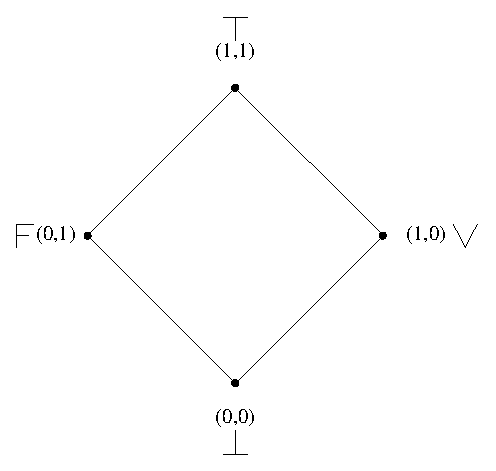
\includegraphics[scale=1.0]{./imagens/C421reticuladoHasse.eps}
\label{fig:reticuladoHasse}

{\small Fonte: \cite{JoaoInacio} }
\end{figure}

Para toda proposição $P$ há um par de valores, chamada de anotação, $(\mu , \lambda )$, onde $\mu$ é o grau de evidência favorável e $\lambda $ é o grau de evidência desfavorável, representada como  $P_{( \mu , \lambda )}$ \cite{Abe2014} .

%$P_{( \mu , \lambda )}$
Como exemplificação, para uma proposição $P \equiv$ \emph{"A velocidade de rotação do motor atingiu o valor desejado."}, assume-se dois especialistas para realizarem a leitura dos valores da anotação. Em um sistema físico, os especialistas geralmente são sensores, como neste caso, poderia ser um encoder ou sensor óptico como contador de voltas associado a uma base de tempo.

\begin{itemize}
\item 
$\mu$ = grau de evidência favorável (especialista 1), ou seja, com quanto de certeza, em um intervalo fechado $[0,1]$, sendo 0 para grau nulo de certeza e 1 grau máximo de certeza para a dada proposição $P$;

\item
$\lambda$ = grau de evidência desfavorável (especialista 2), ou seja, com quanto de certeza, em um intervalo fechado $[0,1]$, sendo 0 o grau nulo de certeza à evidência desfavorável e 1 o grau máximo de certeza à evidência desfavorável para a dada proposição $P$.

\end{itemize}


Assim, podemos interpretar da seguinte forma os valores da anotação para as posições extremas do reticulado finito de Hasse:

\begin{itemize}
\item 
$(\mu, \lambda ) = (1,0)$ : Há um grau de evidência favorável total e um grau de evidencia desfavorável nulo, ou seja, a afirmação da proposição é máxima e sua negação é nula, assim,  $P$ é \emph{Verdadeira} e \emph{A velocidade de rotação do motor atingiu o valor desejado};

\item 
$(\mu, \lambda ) = (0,1)$ : Há um grau de evidência favorável nulo e um grau de evidencia desfavorável máximo, ou seja, a afirmação da proposição é nula e sua negação é máxima, assim,  $P$ é \emph{Falsa} e \emph{A velocidade de rotação do motor não atingiu o valor desejado};

\item 
$(\mu, \lambda ) = (1,1)$ : Há um grau de evidência favorável máximo e também um grau de evidencia desfavorável máximo, ou seja, a afirmação da proposição é máxima e sua negação também é máxima, assim,  $P$ é \emph{Inconsistente} e \emph{A velocidade de rotação do motor atingiu e não atigiu o valor desejado}, contradição;

\item 
$(\mu, \lambda ) = (0,0)$ : Há um grau de evidência favorável nulo e também um grau de evidencia desfavorável nulo, ou seja, a afirmação da proposição é nula e sua negação também é nula, assim,  $P$ é \emph{Indeterminada} e \emph{A velocidade de rotação do motor nem atingiu o valor desejado e nem não atingiu o valor desejado}, situação paracompleta.

\end{itemize}

Os graus de evidência podem assumir valores não extremos:

\begin{itemize}
\item 
$(\mu, \lambda ) = (0.8,0.3)$ : Crê-se com grau de evidência favorável de 80\% e um grau de evidencia desfavorável de 30\%  que \emph{A velocidade rotação do motor atingiu do valor desejado}.
\end{itemize}

\subsubsection{Operações Lógicas}

Algumas operações lógicas booleanas são definidas 
\cite{JISFeAS} \cite{Abe2014}
a partir de duas anotações 
$(\mu _1, \lambda _1)$ e $(\mu _2, \lambda _2)$ 
pertencentes a mesma proposição P, 
aqui denominadas respectivamente $P_1$ e $P_2$:

\begin{itemize}

\item Negação: $\sim$$P _1$ = $(\lambda _1, \mu _1)$ ou 
$\neg$$P _1$ = $(\lambda _1, \mu _1)$

\item Disjunção: $P _1 \vee P _2 = 
(min\{\mu _1, \mu _2\},max\{\lambda _1, \lambda _2\})$ 

\item Conjunção: $P _1 \wedge P _2 = 
(max\{\mu _1, \mu _2\},min\{\lambda _1, \lambda _2\})$ 


\end{itemize}




%%%%%%%%%%%%%%%%%%%%%%%%%%%%%%%%%%%%%%%%%%%%%%%%%%%%%%%%%%%%
\subsection{Quadrado Unitário no Plano Cartesiano - QUPC}
%%%%%%%%%%%%%%%%%%%%%%%%%%%%%%%%%%%%%%%%%%%%%%%%%%%%%%%%%%%%

Uma outra forma de representação da anotação é utilizando o Quadrado Unitário no Plano Cartesiano (QUPC) no qual são transpostos os pontos extremos às respectivas posições de acordo com o par ordenado,  $(\mu, \lambda ) \leftrightarrow (x,y) $, assim o eixo $x$ corresponde ao grau de evidência favorável e o eixo $y$ corresponde ao grau de evidência desfavorável, conforme mostrado na Figura \ref{fig:reticuladoQUPC}.



\begin{figure}[!htb]
\caption{Representação do reticulado no quadrado unitário no plano cartesiano}
\center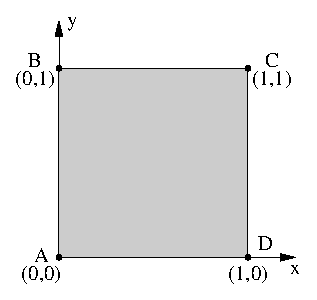
\includegraphics[scale=1.0]{./imagens/C422qupc.eps}
\label{fig:reticuladoQUPC}

{\small Fonte: \cite{JoaoInacio} }
\end{figure}

Os pontos extremos assim representam:

\begin{itemize}
\item $A: (0,0) = \bot \Rightarrow $ Paracompleto;
\item $B: (0,1) = F \Rightarrow $ Falso;
\item $C: (1,1) = \top \Rightarrow $ Contradição;
\item $D: (1,0) = V \Rightarrow $ Verdade.
\end{itemize}

O segmento de reta $\overline{BD}$, entre os pontos referentes às condições $Verdade$ e $Falso$, conforme mostrado na Figura \ref{fig:retaPerfeitamenteDefinida}, é denominada de \emph{Reta Perfeitamente Definida} e dada uma anotação $(\mu, \lambda )$ situada nela, a soma das evidências anotadas é sempre o valor unitário do quadro. 

\begin{figure}[!htb]
\caption{Representação da Reta Perfeitamente Definida}
\center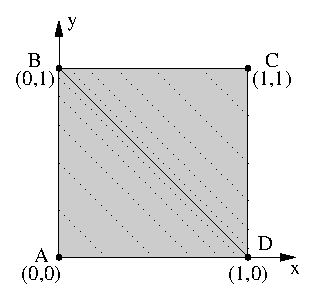
\includegraphics[scale=1.25]{./imagens/C424retaPerfeitamenteDefinida.eps}
\label{fig:retaPerfeitamenteDefinida}

{\small Fonte: \cite{JoaoInacio}}
\end{figure}

A relação dos graus de evidência da anotação quando coincidente à Reta Perfeitamente Definida é: 

\begin{center}
\begin{equation}
\mu + \lambda = 1
\label{eq:evidenciaUnitaria1}
\end{equation}
\end{center}

Assim, temos que:

\begin{center}
\begin{equation}
\mu + \lambda - 1 = 0
\label{eq:evidenciaUnitaria}
\end{equation}
\end{center}


Os graus de evidência não precisam apresentar valores complementares, possuem independência entre si, assim das Equações  
\ref{eq:evidenciaUnitaria1} e 
\ref{eq:evidenciaUnitaria} 
é elaborado o conceito de 
\emph{Grau de Contradição}($G_{ct}$), 
e temos que: 

\begin{center}
\begin{equation}
G _{ct} = \mu + \lambda - 1
\label{eq:grauContradicao}
\end{equation}
\end{center}

pois quanto mais próximo da Reta Perfeitamente Definida, menor é o grau de contradição apresentado pelos graus de evidência, sendo zero quando não houver contradição e o ponto de anotação situar-se sobre a Reta Perfeitamente Definida. 
Quanto mais afastado da Reta Perfeitamente Definida estiver o ponto de anotação, e mais próximo aos pontos A ou C, maior é o Grau de Contradição. 

Quando a anotação estiver situada na região entre os pontos BCD, acima da reta perfeitamente definida, o Grau de Contradição é denominado 
\emph{Grau de Inconsistência} ($G_{it}$), 
e isso ocorre quando, $\mu \ge \lambda $, de forma oposta, quando $\mu < \lambda $ a anotação está situada na região entre os pontos BAD, abaixo da reta perfeitamente definida, e o grau de contradição é denominado 
\emph{Grau de Indefinição} ($G_{id}$), 
então pode-se dizer que:

\begin{center}
\begin{equation}
-1 \le G _{id}  <  0 \le G _{it} \le 1
\label{eq:grauInconsistenciaIndefinicao}
\end{equation}
\end{center}
e
\begin{center}
\begin{equation}
-1 \le G _{ct} \le 1
\label{eq:grauInconsistenciaIndefinicao1}
\end{equation}
\end{center}


O segmento de reta $\overline{ AC }$ , entre os pontos referentes às condições \emph{Paracompleto} e \emph{Contradição}, conforme mostrado na Figura \ref{fig:retaPerfeitamenteIndefinida}, é denominada de \emph{Reta Perfeitamente Indefinida} e dada uma anotação $(\mu, \lambda )$ situada nela, a subtração das evidências anotadas é sempre zero, $\mu = \lambda$, e de forma contrária, quando a anotação está posicionada de forma não coincidente à Reta Perfeitamente Indeterminada, significa que $\mu \neq \lambda$.

\begin{figure}[!htb]
\caption{Representação da Reta Perfeitamente Indefinida}
\center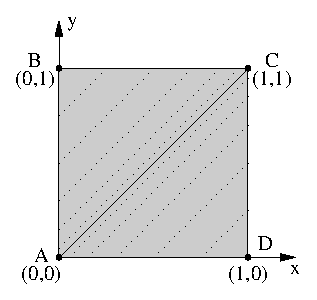
\includegraphics[scale=1.25]{./imagens/C426retaPerfeitamenteIndefinida.eps}
\label{fig:retaPerfeitamenteIndefinida}

{\small Fonte: \cite{JoaoInacio} }
\end{figure}

A relação dos graus de evidência para uma anotação cuja posição coincide com a Reta Perfeitamente Indefinida é: 

\begin{center}
\begin{equation}
\mu - \lambda = 0
\label{eq:evidenciaIndefinida}
\end{equation}
\end{center}

De forma análoga ao Grau de Contradição, da Equação \ref{eq:evidenciaIndefinida} é elaborado o conceito de \emph{Grau de Certeza} ($G _c$), assim temos que: 

\begin{center}
\begin{equation}
G _{c} = \mu - \lambda
\label{eq:grauCerteza}
\end{equation}
\end{center}

Quando os graus de evidência, favorável e desfavorável, são iguais, não há certeza em relação à proposição, mas quando são diferentes, alguma certeza pode ser inferida, até a condição máxima onde uma das evidências é total (1) e a outra é nula (0), caracterizando a condição verdadeira ou falsa, afastando o ponto anotado da Reta Perfeitamente Indefinida. 

Quando a anotação situa-se entre os pontos ABC do QUPC, o grau de certeza é denominado \emph{Grau de Falsidade ($G _f$)}, e tal condição ocorre quando $\mu < \lambda $, caso contrário, se $\mu \ge \lambda $, a anotação situa-se entre os pontos ACD do QUPC, e o grau de certeza é denominado \emph{Grau de Verdade ($G _v)$}, então pode-se dizer que:
\begin{center}
\begin{equation}
-1 \le G _{f}  <  0 \le G _{v} \le 1
\label{eq:grauVerdadeFalsidade}
\end{equation}
\end{center}
e
\begin{center}
\begin{equation}
-1 \le G _{c} \le 1
\label{eq:grauCertezaIntervalo}
\end{equation}
\end{center}

Graficamente são representadas como mostra a Figura \ref{fig:retasgcgct}:

\begin{figure}[!htb]
\caption{Representação dos Graus de Certeza e Contradição em um plano cartesiano}
\center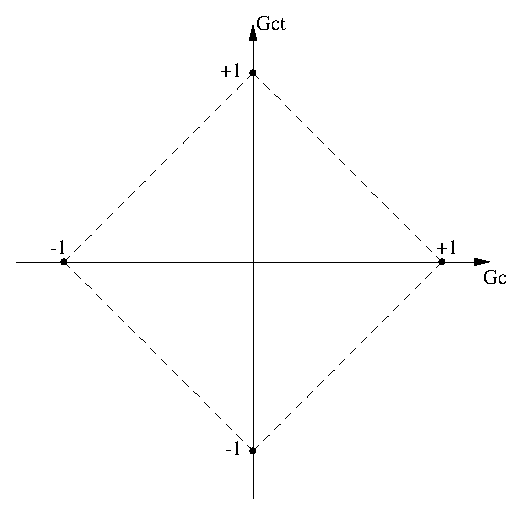
\includegraphics[scale=1.0]{./imagens/C428retasgcgct.eps}
\label{fig:retasgcgct}

{\small Fonte: \cite{JoaoInacio}}
\end{figure}

A representação ainda é dividia em algumas partes, dependendo da aplicação, estabelecendo quais são os limites que definem cada estado, Verdadeiro, Falso, Paracompleto, Contradição e outros mais que forem pertinentes à aplicação, estão representados pelas linhas tracejadas na Figura \ref{fig:valorControle} e são definidos como:

\begin{itemize}
\item \emph{V $_{scc}$ : Valor limite superior de Controle de Certeza};
\item \emph{V $_{icc}$ : Valor limite inferior de Controle de Certeza};
\item \emph{V $_{sci}$ : Valor limite superior de Controle de Incerteza};
\item \emph{V $_{sci}$ : Valor limite inferior de Controle de Incerteza}.

\end{itemize}

\begin{figure}[!htb]
\caption{Representação dos valores de controle}
\center\includegraphics[scale=1.0]{./imagens/C429valorControle.eps}
\label{fig:valorControle}

{\small Fonte: \cite{JoaoInacio}}
\end{figure}

Uma divisão em 12 partes é mostrada na Figura \ref{fig:reticuladoLPA2v} com seus respectivos estados intermediários definidos conforme \citeauthor{JoaoInacio}(\citeyear{JoaoInacio}), sendo 4 regiões extremas:


%\begin{figure}[!htb]
%\center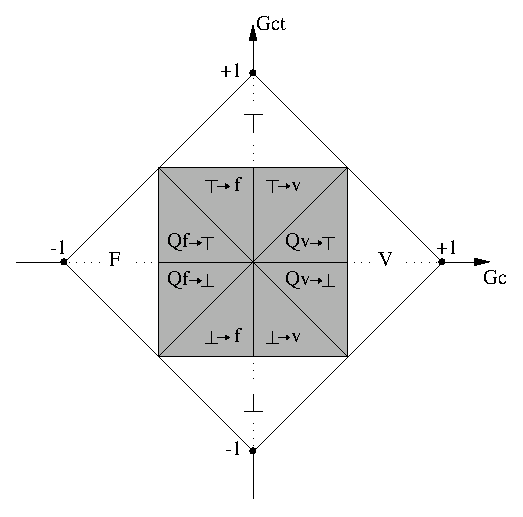
\includegraphics[scale=1.5]{./pic/C430gcgct.eps}
%\caption{Representação do reticulado da LPA2v subdividido em 12 regiões}
%\label{fig:reticuladoLPA2v}
%\end{figure}


\begin{figure}[!h]
\centering
\caption{Representação do reticulado da Lógica $E\tau$ subdividido em 12 regiões}
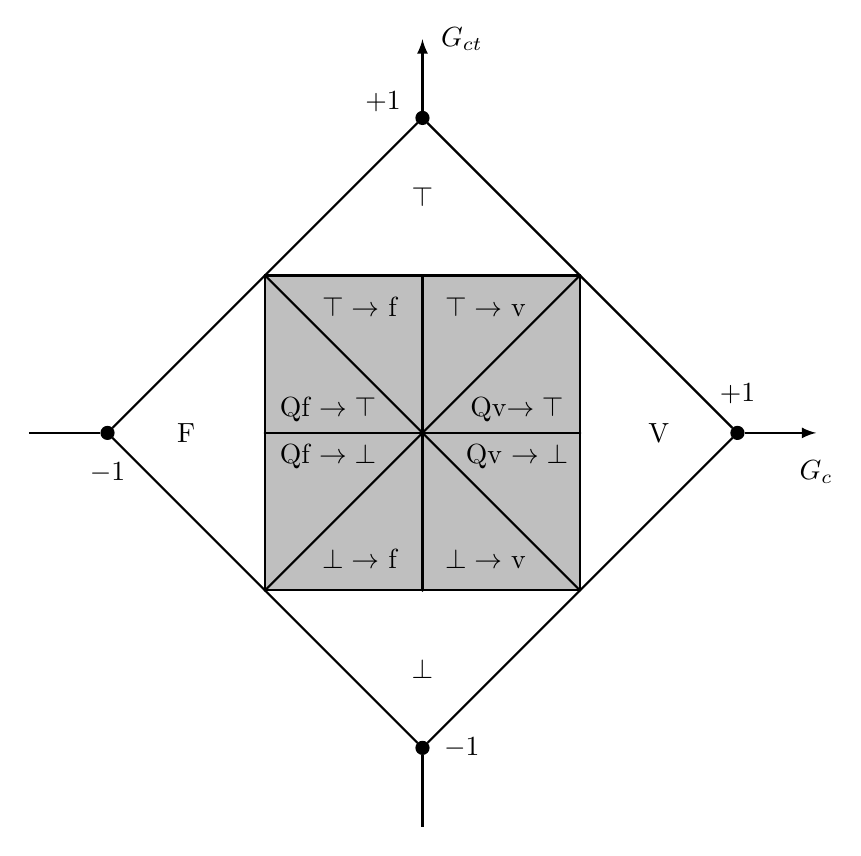
\begin{tikzpicture}[scale=1.0]
\tikzset{ >=latex, inner sep=0pt, outer sep=0pt,  }

%\draw [lightgray, dashed](0,0) grid (10,10);

\node [fill=black, circle] (V) at (9,5) {:};
\node [fill=black, circle] (F) at (1,5) {:};
\node [fill=black, circle] (T) at (5,9) {:};
\node [fill=black, circle] (L) at (5,1) {:};

\node [fill=black, circle] (N) at (5,7) { };
\node [fill=black, circle] (S) at (5,3) { };
\node [fill=black, circle] (E) at (7,5) { };
\node [fill=black, circle] (W) at (3,5) { };

\node [fill=black, circle] (NE) at (7,7) { };
\node [fill=black, circle] (SE) at (7,3) { };
\node [fill=black, circle] (NW) at (3,7) { };
\node [fill=black, circle] (SW) at (3,3) { };


%\draw [dashed] (F) -- (V);
%\draw [dashed] (T) -- (L);
\draw [->, thick] (V)   -- (10,5);
\draw [    thick] (0,5) -- (F);
\draw [->, thick] (T)   -- (5,10);
\draw [    thick] (5,0) -- (L);

\draw [thick] (V) -- (T);
\draw [thick] (T) -- (F);
\draw [thick] (F) -- (L);
\draw [thick] (L) -- (V);

\draw [thick] (N) -- (S);
\draw [thick] (E) -- (W);
\draw [thick] (NE) -- (SW);
\draw [thick] (SE) -- (NW);


\draw[thick] (SW) rectangle (NE);
\fill[nearly transparent] (SW) rectangle (NE);

\node at (8,5) {V};
\node at (2,5) {F};
\node at (5,8) {$\top$};
\node at (5,2) {$\bot$};

\node at (6.2,5.3) {Qv$\rightarrow\top$ };
\node at (6.2,4.7) {Qv $\rightarrow  \bot$ };
\node at (3.8,5.3) {Qf $\rightarrow  \top$ };
\node at (3.8,4.7) {Qf $\rightarrow  \bot$ };
\node at (4.2,6.6) {$\top \rightarrow $ f };
\node at (5.8,6.6) {$\top \rightarrow $ v };
\node at (4.2,3.4) {$\bot \rightarrow $ f };
\node at (5.8,3.4) {$\bot \rightarrow $ v };

\node at (10,4.5) {$G_{c}$};
\node at (5.5,10) {$G_{ct}$};

\node at (4.5,9.2) {$+1$};
\node at (9.0,5.5) {$+1$};
\node at (5.5,1.0) {$-1$};
\node at (1.0,4.5) {$-1$};

\end{tikzpicture}
\label{fig:reticuladoLPA2v}

{\small Fonte: \cite{JoaoInacio} }
\end{figure}




\begin{itemize}
\item V : Verdadeiro;
\item F : Falso;
\item $\top$ : Contradição;
\item $\bot$ : Paracompleto.
\end{itemize}
e 8 regiões intermediárias: 
\begin{itemize}
\item Qv $\rightarrow  \top$ : Quase Verdade tendendo à Contradição;
\item Qv $\rightarrow  \bot$ : Quase Verdade tendendo à  Paracompleto;
\item Qf $\rightarrow  \top$ : Quase Falso tendendo à Contradição;
\item Qf $\rightarrow  \bot$ : Quase Falso tendendo à Paracompleto;
\item $\top \rightarrow $ f : Contradição tendendo à Falso;
\item $\top \rightarrow $ v : Contradição tendendo à Verdadeiro;
\item $\bot \rightarrow $ f : Paracompleto tendendo à Falso;
\item $\bot \rightarrow $ v : Paracompleto tendendo à Verdadeiro.

\end{itemize}

O reticulado subdividido em 12 regiões como mostrado, é aplicado em situações nas quais a tomada de decisão utiliza estados discretos bem definidos para atuação, onde para cada posição da anotação e respectivamente um estado do reticulado, uma ação é tomada, assim sendo, a quantidade de subdivisões está fortemente dependente da aplicação.


O reticulado pode ser dividido de outras formas, dependendo dos limites dos Graus de Certeza e Contradição que o sistema permite. A Figura \ref{fig:reticuladoLPA2v2} mostra uma das possibilidades com a representação de 8 regiões do reticulado. 


\begin{figure}[!h]
\centering
\caption{Representação do reticulado da Lógica $E\tau$ subdividido em 8 regiões}
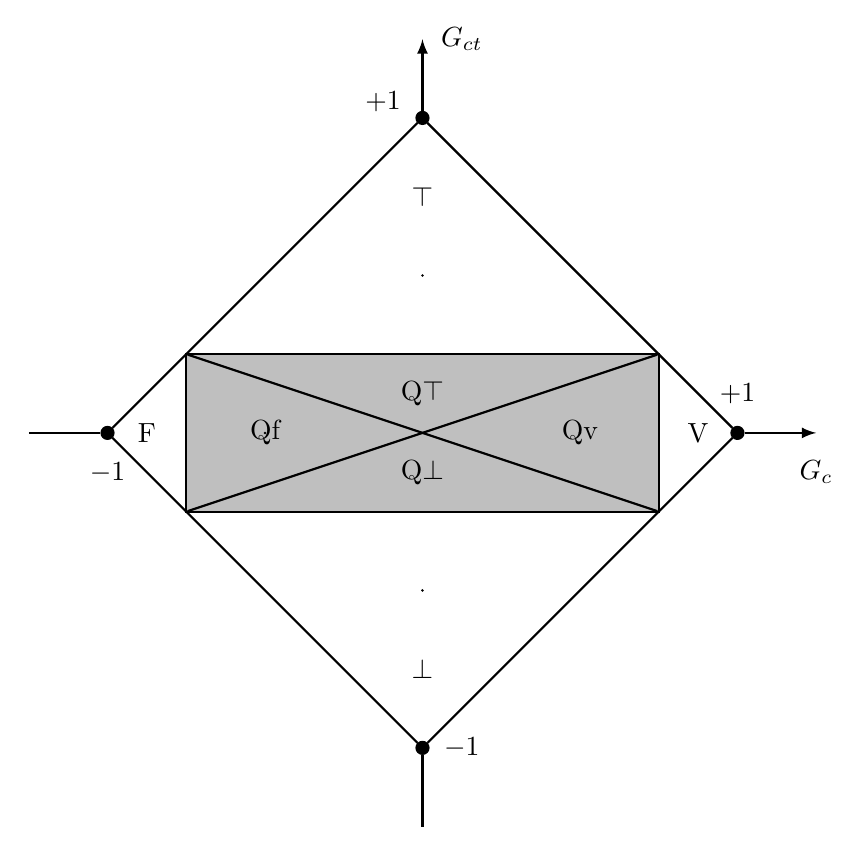
\begin{tikzpicture}[scale=1.0]
\tikzset{ >=latex, inner sep=0pt, outer sep=0pt,  }

%\draw [lightgray, dashed](0,0) grid (10,10);

\node at (10,4.5) {$G_{c}$};
\node at (5.5,10) {$G_{ct}$};

\node at (4.5,9.2) {$+1$};
\node at (9.0,5.5) {$+1$};
\node at (5.5,1.0) {$-1$};
\node at (1.0,4.5) {$-1$};

\node [fill=black, circle] (V) at (9,5) {:};
\node [fill=black, circle] (F) at (1,5) {:};
\node [fill=black, circle] (T) at (5,9) {:};
\node [fill=black, circle] (L) at (5,1) {:};

\node [fill=black, circle] (N) at (5,7) { };
\node [fill=black, circle] (S) at (5,3) { };
\node [fill=black, circle] (E) at (7,5) { };
\node [fill=black, circle] (W) at (3,5) { };

\node [fill=black, circle] (NE) at (8,6) { };
\node [fill=black, circle] (SE) at (8,4) { };
\node [fill=black, circle] (NW) at (2,6) { };
\node [fill=black, circle] (SW) at (2,4) { };

\draw [->, thick] (V)   -- (10,5);
\draw [    thick] (0,5) -- (F);
\draw [->, thick] (T)   -- (5,10);
\draw [    thick] (5,0) -- (L);

\draw [thick] (V) -- (T);
\draw [thick] (T) -- (F);
\draw [thick] (F) -- (L);
\draw [thick] (L) -- (V);

\draw [thick] (NE) -- (SW);
\draw [thick] (SE) -- (NW);

\draw[thick] (SW) rectangle (NE);
\fill[nearly transparent] (SW) rectangle (NE);

\node at (8.5,5.0) {V};
\node at (1.5,5.0) {F};
\node at (5.0,8.0) {$\top$};
\node at (5.0,2.0) {$\bot$};

\node at (7.0,5.0) {Qv};
\node at (3.0,5.0) {Qf};
\node at (5.0,5.5) {Q$\top$};
\node at (5.0,4.5) {Q$\bot$};

\end{tikzpicture}
\label{fig:reticuladoLPA2v2}

{\small Fonte: Próprio autor}
\end{figure}

Sendo 4 regiões extremas,
\begin{itemize}
\item V : Verdadeiro;
\item F : Falso;
\item $\top$ : Contradição;
\item $\bot$ : Paracompleto.
\end{itemize}
e 4 regiões intermediárias: 
\begin{itemize}
\item Qv: Quase Verdade;
\item Qf: Quase Falso;
\item Q$\top$: Quase Contradição;
\item Q$\bot$: Quase Paracompleto.

\end{itemize}


%###

É possível e desejável que se possa utilizar um valor resultante que exclua os efeitos das incertezas ou contradições, 
como é citado por 
\citeauthor{JairJoaoGermano}(\citeyear{JairJoaoGermano}): 
\begin{citacao}
{
"Um sistema de decisão capaz de analisar dados originários de Conhecimento Incerto terá maior robustez quando, 
ao final da análise,
apresentar um resultado que represente o valor de certeza puro, 
isto é, não contaminado pelos efeitos das incertezas."
}
\end{citacao}

O valor que elimina o efeito da incerteza é denominado \emph{Grau de Certeza Real - G$_{CR}$} 
e é calculado pela distância (D) do Ponto de análise, $(G_c,G_{ct})$, 
em relação ao ponto de máximo Grau de Certeza $V$, 
no vértice direito do reticulado, 
conforme mostrado na Figura \ref{fig:reticuladoGer}.


\begin{figure}[!h]
\centering
\caption{Representação do Grau de Certeza Real no reticulado }
\begin{tikzpicture}[scale=1.0]
\tikzset{ >=latex, inner sep=0pt, outer sep=0pt,  }

%\draw [lightgray, dashed](0,0) grid (10,10);

\node at (10,4.5) {$G_{c}$};
\node at (5.5,10) {$G_{ct}$};

\node at (4.5,9.2) {$+1$};
\node at (9.0,5.5) {$+1$};
\node at (5.5,1.0) {$-1$};
\node at (1.0,4.5) {$-1$};

\node at (9.0,4.5) {V};
\node at (1.0,5.5) {F};
\node at (5.5,9.0) {$\top$};
\node at (4.5,1.0) {$\bot$};

\node [fill=black, circle] (V) at (9,5) {:};
\node [fill=black, circle] (F) at (1,5) {:};
\node [fill=black, circle] (T) at (5,9) {:};
\node [fill=black, circle] (L) at (5,1) {:};

\draw [thick] (V) -- (T);
\draw [thick] (T) -- (F);
\draw [thick] (F) -- (L);
\draw [thick] (L) -- (V);

\draw [->, thick] (V)   -- (10,5);
\draw [    thick] (0,5) -- (F);
\draw [->, thick] (T)   -- (5,10);
\draw [    thick] (5,0) -- (L);

\draw [lightgray,dashed] (V) -- (F);
\draw [lightgray,dashed] (T) -- (L);

\node [fill=black, circle] (P) at (6.0,7.0) {:};
\node [fill=gray,  circle] (p) at (5.4,5.0) [gray] {:};
\node [fill=black, circle] (r) at (6.0,5.0) [gray]{.};

\draw [blue,ultra thick] (P) -- (V);
\draw [green ] (r) -- (V);
\draw [yellow] (P) -- (r);
%\draw [green,ultra thick] (9.0,4.9) -- (5.4,4.9);

\draw [red, ultra thick,<-]  (p) to [out=85, in=236] (P);

\node at (7.0,6.0) [blue]{D};
\node at (5.7,7.4) {($G_c$,$G_{ct}$)};
\node at (5.5,4.6) {$G_{CR}$};

\end{tikzpicture}
\label{fig:reticuladoGer}

{\small Fonte: \cite{JairJoaoGermano}}
\end{figure}


O Grau de Certeza Real ($G_{CR}$) 
é calculado utilizando o Teorema de Pitágoras para achar a distância D 
conforme Equação \ref{eq:grauCertezaReal}. 

\begin{center}
\begin{equation}
D = \sqrt{(1-|G_c|)^2+G_{ct}^2}
\label{eq:grauCertezaReal}
\end{equation}
\end{center}

Para valores de $G_c \geq 0$: 

\begin{center}
\begin{equation}
G_{CR} = (1-D)
\end{equation}
\end{center}

Para valores de $G_c < 0$:

\begin{center}
\begin{equation}
G_{CR} = (D-1)
\end{equation}
\end{center}


O Grau de Evidência Real é representado por $\mu_{ER}$ 
e é utilizado para converter o $Gc$ ou $G_{CR}$ 
em uma variável dentro do intervalo fechado $[0,1]$, 
permitindo que o resultado de um bloco LPA$E\tau$ 
possa ser utilizado como entrada em outro bloco. 
Para a conversão é efetuada a equação \ref{eq:muer}:

\begin{equation}
\mu_{ER} = \frac{Gc + 1}{2}
\label{eq:muer}
\end{equation}


Tanto o Grau de Certeza Real quanto o Grau de Evidência Real 
ou os estados ou regiões do reticulado 
podem ser utilizados para realizar o controle dos mais diversos tipos de sistemas, 
dependendo apenas do tipo de controle e de sistema que deve ser implementado. 











%%%%%%%%%%%%%%%%%%%%%%%%%%%%%%%%%%%%%%%%%%%%%%%%%%%%%%%%%%%%
%%%%%%%%%%%%%%%%%%%%%%%%%%%%%%%%%%%%%%%%%%%%%%%%%%%%%%%%%%%%
\section{A proposição e a anotação}

Como ponto de partida, 
dado o sistema a ser controlado apresentado anteriormente, 
tendo como variável controlada 
a velocidade de rotação do disco acoplado ao eixo do motor e 
a variável manipilada o \emph{duty cycle} do sinal \emph{PWM} aplicado ao motor,
a proposição adotada então foi: 
"P: A velocidade de rotação é máxima."

Tal proposição permite que toda extensão de velocidades 
seja representa pelos Graus de evidência.

Os graus de evidência adotados são: 

\begin{itemize}
\item Grau de evidência favorável 0 ($\mu_0$): 
O valor de referência, ou seja, 
o valor desejado para a velocidade de rotação do 
disco acoplado ao eixo do motor(sistema),
também chamado de \emph{setpoint}.
\item Grau de evidência favorável 1 ($\mu_1$): 
O valor lido pelo sensor de rotação, ou seja, a variável controlada.
Esse valor é convertido em 
Grau de evidência desfavorável($\lambda$),
para os devidos cálculos da LPA$E\tau$.
\end{itemize}

O diagrama da Figura \ref{fig:diagramaBlocosLPAEt} apresenta 
a planta do sistema $g(t)$ tendo como saída a 
variável controlada $c(t)$, 
que é a velocidade de rotação do disco 
acoplado ao eixo do motor, 
e como entrada a variável manipulada $u(t)$, 
que é o parâmetro do \emph{PWM} 
que produz a sinal aplicado à planta.



\begin{figure}[!h]%%%%%%%%%%%%%%%%%%%%%%%%%%%%%%%%fg
\centering
\caption{Diagrama de blocos do controle utilizando a LPA$E\tau$}
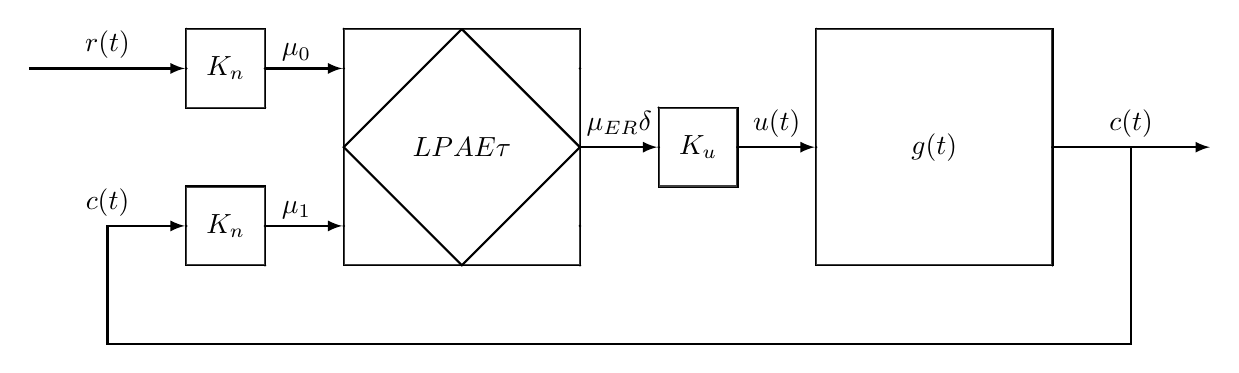
\begin{tikzpicture}[scale=1.0]
\tikzset{ >=latex, inner sep=0pt, outer sep=0pt,  }

%\draw [lightgray, dashed](0,0) grid (15,4.2);

%%% Blocos 

% Kn normalização rps -> 0..1
\node [fill=black, circle] (KSP0) at (2.0,4.0) { };
\node [fill=black, circle] (KSP1) at (3.0,3.0) { };
\draw[thick] (KSP0) rectangle (KSP1);
\fill[white, nearly transparent] (KSP0) rectangle (KSP1);
\node [fill=black, circle] (KSPin)  at (2.0,3.5) { }; 
\node [fill=black, circle] (KSPout) at (3.0,3.5) { }; 
\node (Kn1) at (2.5,3.5) {$K_n$};

% Kn Sensor
\node [fill=black, circle] (KS0) at (2.0,2.0) { };
\node [fill=black, circle] (KS1) at (3.0,1.0) { };
\draw[thick] (KS0) rectangle (KS1);
\fill[white, nearly transparent] (KS0) rectangle (KS1);
\node [fill=black, circle] (KSin)  at (2.0,1.5) { };
\node [fill=black, circle] (KSout) at (3.0,1.5) { };
\node (Kn2) at (2.5,1.5) {$K_n$};

% LPAEt
\node [fill=black, circle] (LPA0) at (4,4.0) { };
\node [fill=black, circle] (LPA1) at (7,1.0) { };
\draw[thick] (LPA0) rectangle (LPA1);
\fill[white, nearly transparent] (LPA0) rectangle (LPA1);
\draw [thick] (5.5,4.0) -- (7.0,2.5) -- (5.5,1.0) -- (4.0,2.5) -- (5.5,4.0);
\node (LPA2v) at (5.5,2.5) {$LPAE\tau$};
\node [fill=black, circle] (LPAu0)  at (4.0,3.5) { };
\node [fill=black, circle] (LPAu1)  at (4.0,1.5) { };
\node [fill=black, circle] (LPAgc)  at (7.0,3.5) { };
\node [fill=black, circle] (LPAs)   at (7.0,2.5) { };
\node [fill=black, circle] (LPAgct) at (7.0,1.5) { };
\node (LPA2vu0)  at (3.4,3.7) {$\mu _0$};
\node (LPA2vu1)  at (3.4,1.7) {$\mu _1$};

% Kn u(t)
\node [fill=black, circle] (KU0) at (8.0,3.0) { };
\node [fill=black, circle] (KU1) at (9.0,2.0) { };
\draw[thick] (KU0) rectangle (KU1);
\fill[white, nearly transparent] (KU0) rectangle (KU1);
\node [fill=black, circle] (KUin)  at (8.0,2.5) { };
\node [fill=black, circle] (KUout) at (9.0,2.5) { };
\node (Ku2) at (8.5,2.5) {$K_u$};


% Planta
\node [fill=black, circle] (GT0) at (10,4.0) { };
\node [fill=black, circle] (GT1) at (13,1.0) { };
\draw[thick] (GT0) rectangle (GT1);
\fill[white, nearly transparent] (GT0) rectangle (GT1);
\node [fill=black, circle] (GTin)  at (10.0,2.5) { };
\node [fill=black, circle] (GTout) at (13.0,2.5) { };
\node (planta) at (11.5,2.5) {$g(t)$};



%%% Linhas 

% set point
\draw [->, thick] (0.0,3.5) -- (KSPin);
\node (rt) at (1.0,3.8) {$r(t)$};

% GT -> fim
\draw [->, thick] (GTout) -- (15,2.5);
\node (ct) at (14.0,2.8) {$c(t)$};
\node (ct) at (1.0,1.8) {$c(t)$};

% normalização 0..1 -> LPA2v u0
\draw [->, thick] (KSPout) -- (LPAu0);

% normalização 0..1 -> LPA2v u1
\draw [->, thick] (KSout) -- (LPAu1);

% LPAEt -> Ku
\draw [->, thick] (LPAs) -- (KUin);
\node (ut) at (7.5,2.8) {$\mu_{ER}\delta$};

% Ku -> GT
\draw [->, thick] (KUout) -- (GTin);
\node (ut) at (9.5,2.8) {$u(t)$};

% GT -> Kn Sensor
\draw [->, thick] (GTout) -- (14.0,2.5) -- (14.0,0.0) -- (1.0,0.0) -- (1.0,1.5) -- (KSin);


\end{tikzpicture}
\label{fig:diagramaBlocosLPAEt}

{\vspace{0.2cm} \small Fonte: Próprio autor}
\end{figure}
%%%%%%%%%%%%%%%%%%%%%%%%%%%%%%%%%%%%%%%%



A variável manipulada $u(t)$ é produzida pelo 
bloco controlador $LPAE\tau$, 
e este recebe seus parâmetros no formato dos 
graus de evidência favoráveis $\mu_0$ e $\mu_1$.
Sendo o parâmetro $\mu_1$ 
convertido internamente em $\lambda$ 
como grau de evidência desfavorável.

Os dois parâmetros que vão gerar os graus de evidência 
possuem a mesma natureza, a mesma escala, 
são a velocidade desejada e a velocidade lida pelo sensor,
de mode a poder comparar e utilizá-las nas operações da
LPA$E\tau$. 
Para adequação da escala das grandezas 
de referência $r(t)$ e da variável controlada $c(t)$
ao intervalo de trabalho dos parâmetros da LPA$E\tau$, 
é inserido um bloco de normalização do sinal em cada entrada,
bem como na saída.


Para a normalização os blocos $K_n$ realizam as seguinte operações:

\begin{equation}%%%%%%%%%%%%%%%%%%%%%%%%%%%%%%%%%% eq
\mu_0 = \frac{ r(t)}{c(t)_{\text{máx}}} \ \ \ \ \ \ \ \ \mu_1 = \frac{c(t)}{c(t)_{\text{máx}}}
\end{equation}%%%%%%%%%%%%%%%%%%%%%%%%%%%%%%%%%%%%

onde:

$c(t)_{\text{máx}}$: é a velocidade máxima produzida pelo sistema.


Para a normalização do bloco $K_u$ é realizada a seguinte operação:

\begin{equation}
u(t) = \mu_{ER}\delta . 100
\end{equation}

onde:

$\mu_{ER}\delta$: valor contido no intervalo fechado [0, 1].

$u(t)$: valor contido no intervalo [0, 100] 
referente ao parâmetro(\%) do acionamento PWM.




%%%%%%%%%%%%%%%%%%%%%%%%%%%%%%%%%%%%%%%%%%%%%%%%%%%%%%%%%%%%
%%%%%%%%%%%%%%%%%%%%%%%%%%%%%%%%%%%%%%%%%%%%%%%%%%%%%%%%%%%%
\newpage


\section{Ação de controle Liga-Desliga utilizando a LPA$E\tau$}

Assim como pode ser encontrado em Ação de Controle no Anexo A, 
o tipo mais simples de controlador, o Liga-Desliga,
pode ser implementado utilizando a 
LPA$E\tau$, dividindo o reticulado em duas partes
e sua representação para a condição em que o $Gct$ define o estado
de Ligar ou Desligar o sistema é mostrado na 
Figura \ref{fig:reticuladoEtOnOff}.





%%%%%%%%%%%%%%%%%%%%%%%%%%%%%%%%%%%%%%%%%%%%%%%%%%%%
\begin{figure}[!h]%%%%%%%%%%%%%%%%%%%%%%%%%%%%%%%%fg
\centering
\caption{Representação do reticulado da LPA$E\tau$ dividido em duas partes}
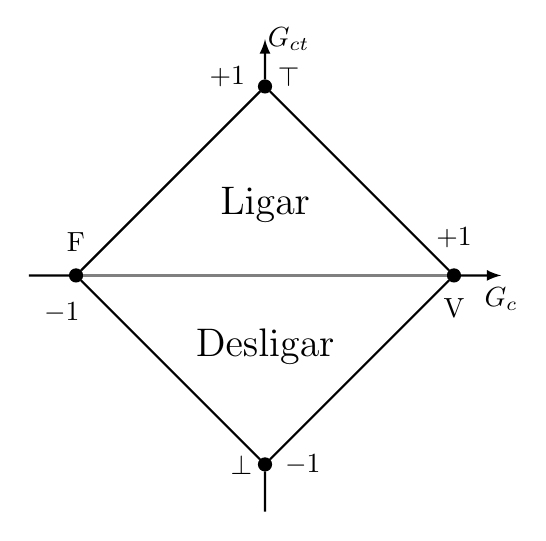
\begin{tikzpicture}[scale=0.60]
\tikzset{ >=latex, inner sep=0pt, outer sep=0pt,  }

%\draw [lightgray, dashed](0,0) grid (10,10);

\node [fill=black, circle] (V) at (9,5) {:};
\node [fill=black, circle] (F) at (1,5) {:};
\node [fill=black, circle] (T) at (5,9) {:};
\node [fill=black, circle] (L) at (5,1) {:};

\draw [->, thick] (V)   -- (10,5);
\draw [    thick] (0,5) -- (F);
\draw [->, thick] (T)   -- (5,10);
\draw [    thick] (5,0) -- (L);

\draw [thick] (V) -- (T);
\draw [thick] (T) -- (F);
\draw [thick] (F) -- (L);
\draw [thick] (L) -- (V);

\draw [gray,thick] (V) -- (F);

\node at (10,4.5) {$G_{c}$};
\node at (5.5,10) {$G_{ct}$};

\node at (4.2,9.2) {$+1$};
\node at (9.0,5.8) {$+1$};
\node at (5.8,1.0) {$-1$};
\node at (0.7,4.2) {$-1$};

\node at (9.0,4.3) {V};
\node at (1.0,5.7) {F};
\node at (5.5,9.2) {$\top$};
\node at (4.5,1.0) {$\bot$};

\node at (5.0,6.5) {\Large{Ligar}};
\node at (5.0,3.5) {\Large{Desligar}};

\end{tikzpicture}
\label{fig:reticuladoEtOnOff}

{\small Fonte: Próprio autor }
\end{figure}%%%%%%%%%%%%%%%%%%%%%%%%%%%%%%%%%%%%%%
%%%%%%%%%%%%%%%%%%%%%%%%%%%%%%%%%%%%%%%%%%%%%%%%%%





Utilizando o $Gct$ como variável condicionante:

\begin{itemize}
\item $Gct > 0 $: 
Para todas as combinaçãos de valores que produzam 
$\mu_0 > \mu_1$, 
ou seja, a variável de referência do sistema é 
maior do que a variável controlada,
o Grau de contradição encontra-se na condição de 
\textit{Inconsistência}, conforme exposto na Equação 
\ref{eq:grauInconsistenciaIndefinicao}.

Substituindo $\mu$ por $\mu_0$ e 
$\lambda$ por $(1-\mu_1)$, 
utilizando a Equação \ref{eq:grauContradicao} 
( $Gct = \mu + \lambda - 1 $ )
temos:



\begin{equation}%%%%%%%%%%%%%%%%%%%%%%%%%%%%%%% Eq
Gct = \mu_0 + (1-\mu_1) -1
\end{equation}%%%%%%%%%%%%%%%%%%%%%%%%%%%%%%%%%%%%



simplificando temos então:



\begin{equation}%%%%%%%%%%%%%%%%%%%%%%%%%%%%%%% Eq
Gct = \mu_0 - \mu_1
\label{eq:gctmu0mu1}
\end{equation}%%%%%%%%%%%%%%%%%%%%%%%%%%%%%%%%%%%%



Supondo que o \emph{especialista 0} afirme que 
o valor da variável controlada é 25\% do valor máximo, 
o grau de evidência favorável 0 é $\mu_0 = 0,25$, 
enquanto que o \emph{especialista 1} afirma que 
seu valor é de 20\% do valor máximo, 
o grau de evidência favorável 1 é $\mu_1 = 0,20$. 
Substituindo $\mu_0$ e $\mu_1$ em \ref{eq:gctmu0mu1}:



\begin{equation}%%%%%%%%%%%%%%%%%%%%%%%%%%%%%%% Eq
Gct = 0,25 - 0,20 = 0,05
\end{equation}%%%%%%%%%%%%%%%%%%%%%%%%%%%%%%%%%%%%



O ponto de operação do sistema 
localiza-se, então, acima da reta perfeitamente definida,
para todo grau de contradição positivo, 
como é mostrado na Figura \ref{fig:gctpos}.



\item $Gct < 0 $: 
Para todas as combinações de valores que produzam 
$\mu_0 < \mu_1$, 
ou seja, a variável de referência do sistema é 
menor do que a variável controlada. 
O Grau de contradição encontra-se na condição de 
\textit{Indefinição}, conforme exposto na Equação 
\ref{eq:grauInconsistenciaIndefinicao}.

Supondo agora que 
\emph{especialista 0} continue afirmando  que 
o valor da variável controlada é 25\% do valor máximo,
o grau de evidência favorável 0 é $\mu_0 = 0,25 = \mu$, 
mas o \emph{especialista 1} afirma agora que
seu valor é de 30\% do valor máximo,
o grau de evidência favorável 2 é $\mu_1 = 0,30$.
Substituindo $\mu_0$ e $\mu_1$ em \ref{eq:gctmu0mu1}:



\begin{equation}%%%%%%%%%%%%%%%%%%%%%%%%%%%%%%% Eq
Gct = 0,25 - 0,30 = -0,05
\end{equation}%%%%%%%%%%%%%%%%%%%%%%%%%%%%%%%%%%%%



O ponto de operação do sistema 
localiza-se, então, abaixo da reta perfeitamente definida,
para todo grau de contradição negativo,
como é mostrado na Figura \ref{fig:gctneg}.




\end{itemize}




%%%%%%%%%%%%%%%%%%%%%%%%%%%%%%%%%%%%%%%%%%%%%%% Fg
\begin{figure}[!htb]%%%%%%%%%%%%%%%%%%%%%%%%%%%%%%
\centering
\caption{Representação do reticulado da LPA$E\tau$ para ação de controle Liga-Desliga}
\subfloat[$Gct$ positivo ($\mu_0 > \mu_1$)]{\label{fig:gctpos}

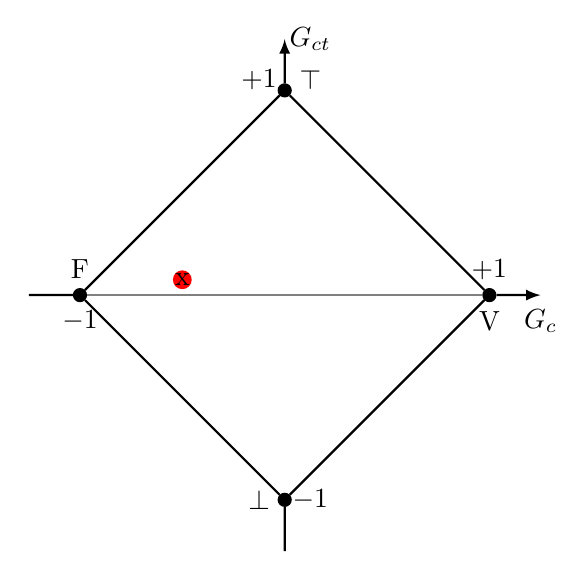
\begin{tikzpicture}[scale=0.65]
\tikzset{ >=latex, inner sep=0pt, outer sep=0pt,  }
%\draw [lightgray, dashed](0,0) grid (10,10);

\node [fill=black, circle] (V) at (9,5) {:};
\node [fill=black, circle] (F) at (1,5) {:};
\node [fill=black, circle] (T) at (5,9) {:};
\node [fill=black, circle] (L) at (5,1) {:};

\draw [->, thick] (V)   -- (10,5);
\draw [    thick] (0,5) -- (F);
\draw [->, thick] (T)   -- (5,10);
\draw [    thick] (5,0) -- (L);

\draw [thick] (V) -- (T);
\draw [thick] (T) -- (F);
\draw [thick] (F) -- (L);
\draw [thick] (L) -- (V);

\draw [gray,thick] (V) -- (F);

\node at (10,4.5) {$G_{c}$};
\node at (5.5,10) {$G_{ct}$};

\node at (4.5,9.2) {$+1$};
\node at (9.0,5.5) {$+1$};
\node at (5.5,1.0) {$-1$};
\node at (1.0,4.5) {$-1$};

\node at (9.0,4.5) {V};
\node at (1.0,5.5) {F};
\node at (5.5,9.2) {$\top$};
\node at (4.5,1.0) {$\bot$};

\node [fill=red, circle] (MU) at (3.0,5.3) {x};

\end{tikzpicture} }
\subfloat[$Gct$ negativo ($\mu_0<\mu_1$)]{\label{fig:gctneg}
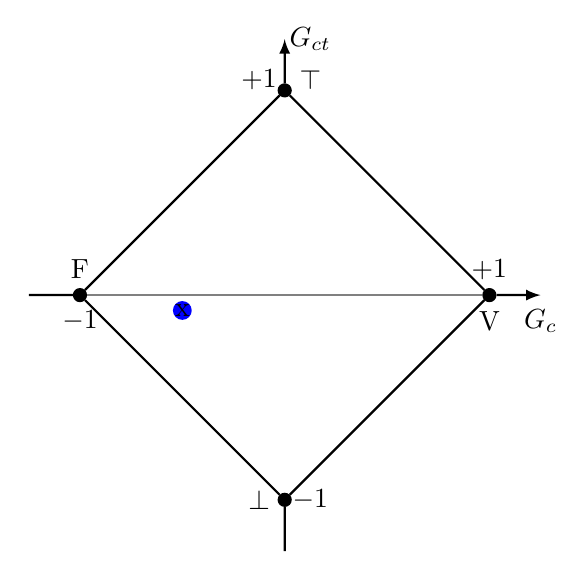
\begin{tikzpicture}[scale=0.65]
\tikzset{ >=latex, inner sep=0pt, outer sep=0pt,  }
%\draw [lightgray, dashed](0,0) grid (10,10);

\node [fill=black, circle] (V) at (9,5) {:};
\node [fill=black, circle] (F) at (1,5) {:};
\node [fill=black, circle] (T) at (5,9) {:};
\node [fill=black, circle] (L) at (5,1) {:};

\draw [->, thick] (V)   -- (10,5);
\draw [    thick] (0,5) -- (F);
\draw [->, thick] (T)   -- (5,10);
\draw [    thick] (5,0) -- (L);

\draw [thick] (V) -- (T);
\draw [thick] (T) -- (F);
\draw [thick] (F) -- (L);
\draw [thick] (L) -- (V);

\draw [gray,thick] (V) -- (F);

\node at (10,4.5) {$G_{c}$};
\node at (5.5,10) {$G_{ct}$};

\node at (4.5,9.2) {$+1$};
\node at (9.0,5.5) {$+1$};
\node at (5.5,1.0) {$-1$};
\node at (1.0,4.5) {$-1$};

\node at (9.0,4.5) {V};
\node at (1.0,5.5) {F};
\node at (5.5,9.2) {$\top$};
\node at (4.5,1.0) {$\bot$};

\node [fill=blue, circle] (MU1) at (3.0,4.7) {x};

\end{tikzpicture}}

\label{fig:sistPrimeiraOrdem}

{\small Fonte: Próprio autor}
\end{figure}%%%%%%%%%%%%%%%%%%%%%%%%%%%%%%%%%%%%%%
%%%%%%%%%%%%%%%%%%%%%%%%%%%%%%%%%%%%%%%%%%%%%%%%%%





Podemos então notar que 
a diferença existente entre os graus de evidência favoráveis 
é equivalente ao erro, 
como é denominado no sistema clássico de controle, 
mas que na LPA$E\tau$ pode ser considerado como 
o Grau de Contradição, pois,
na condição em que a variável controlada é igual a 
variável de referência, não há erro, e a contradição é zero, 
entretando se forem diferentes, 
tanto o erro quanto o grau de contradição
serão não nulos. 

A opção pela ação de controle Liga-Desliga
é interessante do ponto de vista da velocidade 
de resposta ao degrau, 
porém apresenta uma oscilação que, 
a depender da dinâmica do sistema que está sendo trabalhado,
pode gerar uma amplitude maior do que o aceitável.
%como pôde ser visto na 
%Figura \ref{fig:acaoControleLigaDesliga}.

%Outra estratégia simples é a 
%utilização do sistema sem realimentação, 
%aplicando à saída o valor proporcional desejado.


\section{A variável manipulada e a equivalência do controle em malha aberta}

Uma outra estratégia de controle simples, 
é a implementação equivalente a um controle em malha aberta,
onde é aplicado à entrada da planta, 
através da variável manipulada,
um valor proporcional ao valor desejado na saída,
que é a variável controlada, 
porém a planta controlada necessita apresentar um 
comportamento linear. 

Para a implementação da saída do bloco 
LPA$E\tau$ de modo equivalente ao sistema em malha aberta,
assumindo não haver contradição, 
e para a Proposição adotada: 
\emph{"P: A velocidade de rotação é máxima"}, 
temos a Reta Perfeitamente Definida como referencial. 

A Figura \ref{fig:gc25} mostra o ponto de operação 
para uma velocidade de 25\% da proposição, 
e a Figura \ref{fig:gc90} mostra o ponto de operação
para a velocidade de 90\% da proposição.





%%%%%%%%%%%%%%%%%%%%%%%%%%%%%%%%%%%%%%%
%%%%%%%%%%%%%%%%%%%%%%%%%%%%%%%%%%%%%%%



\begin{figure}[!htb]
\centering
\caption{Representação do reticulado da LPA$E\tau$}
\subfloat[$Gc = -0,50 \ \ \ \mu_{ER} = 0,25$]{\label{fig:gc25}

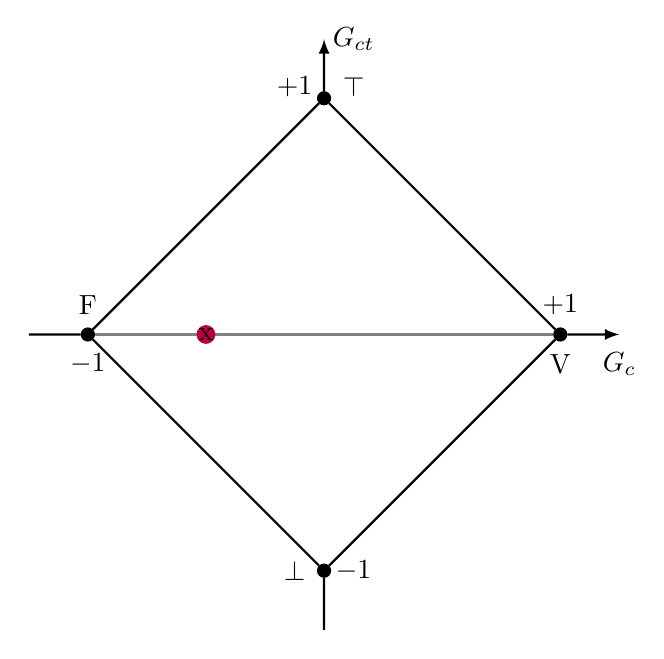
\begin{tikzpicture}[scale=0.75]
\tikzset{ >=latex, inner sep=0pt, outer sep=0pt,  }
%\draw [lightgray, dashed](0,0) grid (10,10);

\node [fill=black, circle] (V) at (9,5) {:};
\node [fill=black, circle] (F) at (1,5) {:};
\node [fill=black, circle] (T) at (5,9) {:};
\node [fill=black, circle] (L) at (5,1) {:};

\draw [->, thick] (V)   -- (10,5);
\draw [    thick] (0,5) -- (F);
\draw [->, thick] (T)   -- (5,10);
\draw [    thick] (5,0) -- (L);

\draw [thick] (V) -- (T);
\draw [thick] (T) -- (F);
\draw [thick] (F) -- (L);
\draw [thick] (L) -- (V);

\draw [gray,thick] (V) -- (F);

\node at (10,4.5) {$G_{c}$};
\node at (5.5,10) {$G_{ct}$};

\node at (4.5,9.2) {$+1$};
\node at (9.0,5.5) {$+1$};
\node at (5.5,1.0) {$-1$};
\node at (1.0,4.5) {$-1$};

\node at (9.0,4.5) {V};
\node at (1.0,5.5) {F};
\node at (5.5,9.2) {$\top$};
\node at (4.5,1.0) {$\bot$};

\node [fill=purple, circle] (MU) at (3.0,5.0) {x};

\end{tikzpicture} }
\subfloat[$Gc = 0,80 \ \ \ \mu_{ER} = 0,90$]{\label{fig:gc90}
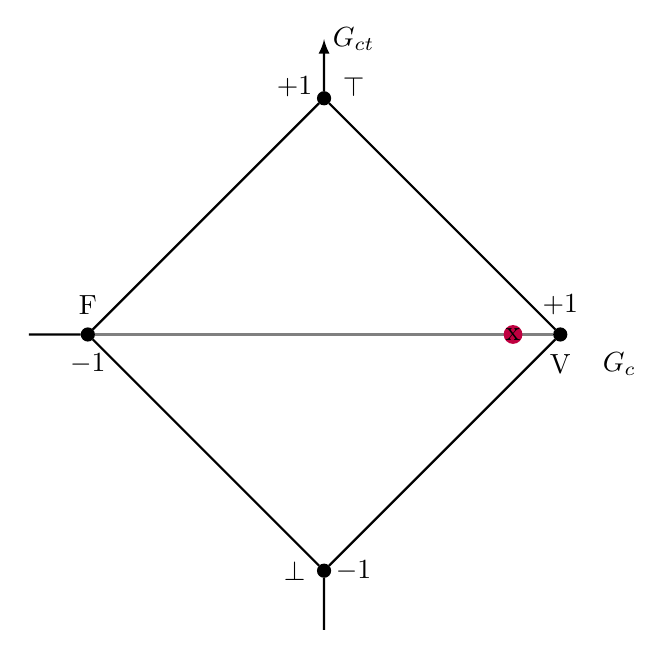
\begin{tikzpicture}[scale=0.75]
\tikzset{ >=latex, inner sep=0pt, outer sep=0pt,  }

\node [fill=black, circle] (V) at (9,5) {:};
\node [fill=black, circle] (F) at (1,5) {:};
\node [fill=black, circle] (T) at (5,9) {:};
\node [fill=black, circle] (L) at (5,1) {:};

\draw [    thick] (0,5) -- (F);
\draw [->, thick] (T)   -- (5,10);
\draw [    thick] (5,0) -- (L);

\draw [thick] (V) -- (T);
\draw [thick] (T) -- (F);
\draw [thick] (F) -- (L);
\draw [thick] (L) -- (V);

\draw [gray,thick] (V) -- (F);

\node at (10,4.5) {$G_{c}$};
\node at (5.5,10) {$G_{ct}$};

\node at (4.5,9.2) {$+1$};
\node at (9.0,5.5) {$+1$};
\node at (5.5,1.0) {$-1$};
\node at (1.0,4.5) {$-1$};

\node at (9.0,4.5) {V};
\node at (1.0,5.5) {F};
\node at (5.5,9.2) {$\top$};
\node at (4.5,1.0) {$\bot$};

\node [fill=purple, circle] (MU1) at (8.2,5.0) {x};

\end{tikzpicture}}

\label{fig:sistPrimeiraOrdem}

{\small Fonte: Próprio autor}
\end{figure}





%%%%%%%%%%%%%%%%%%%%%%%%%%%%%%%%%%%%%%%%%%%%%%%%%%
%%%%%%%%%%%%%%%%%%%%%%%%%%%%%%%%%%%%%%%%%%%%%%%%%%



\vspace{3cm}

Assim, considerando o Grau de Contradição nulo:

\begin{equation}
Gct = \mu + \lambda - 1 = 0 \rightarrow \mu = 1 - \lambda
\end{equation}

como $\mu_1 = 1 - \lambda$ e $\mu = \mu_0$:

\begin{equation}
\mu_0 = \mu_1
\label{eq:mu0eqmu1}
\end{equation}

substituindo $Gc$ por $\mu-\lambda$ e aplicando $\mu_0$ e $\lambda = 1 - \mu_1$ na Eq. \ref{eq:muer}:

\begin{equation}
\mu_{ER} = \frac{Gc + 1}{2} \rightarrow \mu_{ER} = \frac{(\mu_0 + \mu_2 - 1) + 1}{2} \rightarrow \mu_{ER} = \frac{\mu_0 + \mu_1}{2}
\label{eq:uermu0mu1}
\end{equation}

aplicando \ref{eq:mu0eqmu1} em \ref{eq:uermu0mu1}:

\begin{equation}
\mu_{ER} = \frac{\mu_0 + \mu_0}{2} = \frac{2.\mu_0}{2} = \mu_0
\end{equation}


Assim, adota-se como valor para a variável manipulada 
o valor $\mu_{ER}$, que é o próprio valor do 
grau de evidência favorável ($\mu_0$), 
e pode ser exemplificado na 
Figura \ref{fig:gc25} e na 
Figura \ref{fig:gc90}, 
respectivamente para valores de referência de 25\% e 90\%
do valor máximo da variável controlada, 
que é a velocidade de rotação máxima alcançada 
pelo motor no sistema proposto.





%%%%%%%%%%%%%%%%%%%%%%%%%%%%%%%%%%%%%%%%%%%%%%%%%%%%%%%%%%%%
%%%%%%%%%%%%%%%%%%%%%%%%%%%%%%%%%%%%%%%%%%%%%%%%%%%%%%%%%%%%





\section{A região de parada - zona morta}

O sistema possui uma região de operação 
que não é possível realizar o controle, 
pois é a região onde a inércia do sistema parado
impede a movimentação do eixo do motor,
denominada de Zona Morta, 
%o que deixa de acontecer em torno dos 10\% do valor do PWM.
e é estipulado, inicialmente, um valor em torno dos 10\% do valor máximo de rotação.
A Figura \ref{fig:zonaMorta} mostra essa região:





%%%%%%%%%%%%%%%%%%%%%%%%%%%%%%%%%%%%%%%%%%%%%%%%%%%%%%%%% Fg
\begin{figure}[!h]%%%%%%%%%%%%%%%%%%%%%%%%%%%%%%%%%%%%%%%%%%
\centering
\caption{Representação da zona morta no reticulado da LPA$E\tau$}
\begin{tikzpicture}[scale=0.80]
\tikzset{ >=latex, inner sep=0pt, outer sep=0pt,  }

%\draw [lightgray, dashed](0,0) grid (10,10);

\node [fill=black, circle] (V) at (9,5) {:};
\node [fill=black, circle] (F) at (1,5) {:};
\node [fill=black, circle] (T) at (5,9) {:};
\node [fill=black, circle] (L) at (5,1) {:};

\draw [->, thick] (V)   -- (10,5);
\draw [    thick] (0,5) -- (F);
\draw [->, thick] (T)   -- (5,10);
\draw [    thick] (5,0) -- (L);

\draw [thick] (V) -- (T);
\draw [thick] (T) -- (F);
\draw [thick] (F) -- (L);
\draw [thick] (L) -- (V);

\node at (10,4.5) {$G_{c}$};
\node at (5.5,10) {$G_{ct}$};

\node at (4.5,9.2) {$+1$};
\node at (9.0,5.5) {$+1$};
\node at (5.5,1.0) {$-1$};
\node at (1.0,4.5) {$-1$};

\node at (9.0,4.5) {V};
\node at (1.0,5.5) {F};
\node at (5.5,9.2) {$\top$};
\node at (4.5,1.0) {$\bot$};

\draw [fill, red,nearly transparent] (1.0,5.0) -- (1.5,5.5) -- (1.5,4.5) -- (1.0,5.0);
\draw [thick] (5.0,9.0) -- (1.0,5.0);
\draw [gray,thick] (V) -- (F);
\draw [dashed, red] (1.5,5.5) -- (1.5,4.5);
\end{tikzpicture}
\label{fig:zonaMorta}

{\small Fonte: Próprio autor }
\end{figure}
%%%%%%%%%%%%%%%%%%%%%%%%%%%%%%%%%%%%%%%%%%%%%%%%%%%%%%%%%%%%





Outra condição crítica para o sistema é 
quando houver um travamento do eixo do motor,
levando o grau de evidência $\mu_1$ para a condição nula,
ou seja, $\lambda$ para o valor máximo. 
A Figura \ref{fig:travamentoEixo} mostra a região 
que pode sinalizar tal anormalidade.




%%%%%%%%%%%%%%%%%%%%%%%%%%%%%%%%%%%%%%%%%%%%%%% Fg
\begin{figure}[!h]%%%%%%%%%%%%%%%%%%%%%%%%%%%%%%%%
\centering
\caption{Representação da região de travamento no reticulado da LPA$E\tau$}
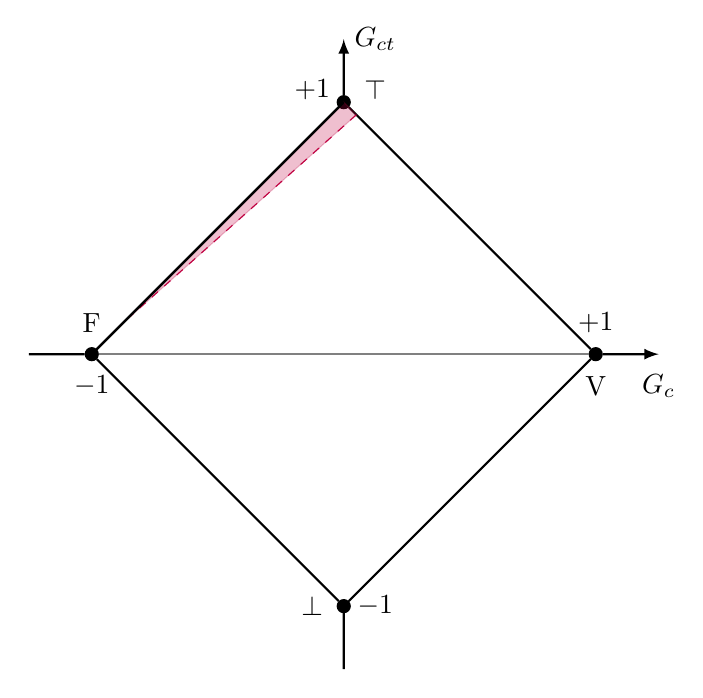
\begin{tikzpicture}[scale=0.80]
\tikzset{ >=latex, inner sep=0pt, outer sep=0pt,  }

%\draw [lightgray, dashed](0,0) grid (10,10);

\node [fill=black, circle] (V) at (9,5) {:};
\node [fill=black, circle] (F) at (1,5) {:};
\node [fill=black, circle] (T) at (5,9) {:};
\node [fill=black, circle] (L) at (5,1) {:};

\draw [->, thick] (V)   -- (10,5);
\draw [    thick] (0,5) -- (F);
\draw [->, thick] (T)   -- (5,10);
\draw [    thick] (5,0) -- (L);

\draw [thick] (V) -- (T);
\draw [thick] (T) -- (F);
\draw [thick] (F) -- (L);
\draw [thick] (L) -- (V);

\node at (10,4.5) {$G_{c}$};
\node at (5.5,10) {$G_{ct}$};

\node at (4.5,9.2) {$+1$};
\node at (9.0,5.5) {$+1$};
\node at (5.5,1.0) {$-1$};
\node at (1.0,4.5) {$-1$};

\node at (9.0,4.5) {V};
\node at (1.0,5.5) {F};
\node at (5.5,9.2) {$\top$};
\node at (4.5,1.0) {$\bot$};

\draw [fill, purple, nearly transparent] (1.5,5.5) -- (5.0,9.0) -- (5.2,8.8) -- (1.5,5.5);
\draw [dashed, purple] (5.2,8.8) -- (1.5,5.5);
\draw [thick] (5.0,9.0) -- (1.0,5.0);
\draw [gray,thick] (V) -- (F);
\end{tikzpicture}
\label{fig:travamentoEixo}

{\small Fonte: Próprio autor }
\end{figure}
%%%%%%%%%%%%%%%%%%%%%%%%%%%%%%%%%%%%%%%%%%%%%%%%%%





Nesta condição o controlador pode tomar a dicisão de 
desligar o sistema controlado, 
levá-lo a condição de falha e 
sinalizar ao operador a irregularidade, 
a depender do tipo de sistema a ser controlado.



\section{ A região de operação }

Para a região de operação, 
foi estipulado um valor de grau de contradição
%para atender os requisitos de desempenho do sistema,
podendo ser alterado posteriormente após testes empíricos.
O grau de contradição está definido entre o intervalo menor do que 0,1 ($Gct < 1$) 
e maior do que -0,05 ($Gct > -0,05$). Assumindo um valor inicial para
a variável manipulada equivalente a um controle em malha aberta, sendo
assim a resposta do controlador é o próprio $\mu_0$ como mostrado na
Figura \ref{fig:regiaoAtiva}.





%%%%%%%%%%%%%%%%%%%%%%%%%%%%%%%%%%%%%%%%%%%%%%% Fg
\begin{figure}[!h]%%%%%%%%%%%%%%%%%%%%%%%%%%%%%%%%
\centering
\caption{Representação da região ativa no reticulado da LPA$E\tau$}
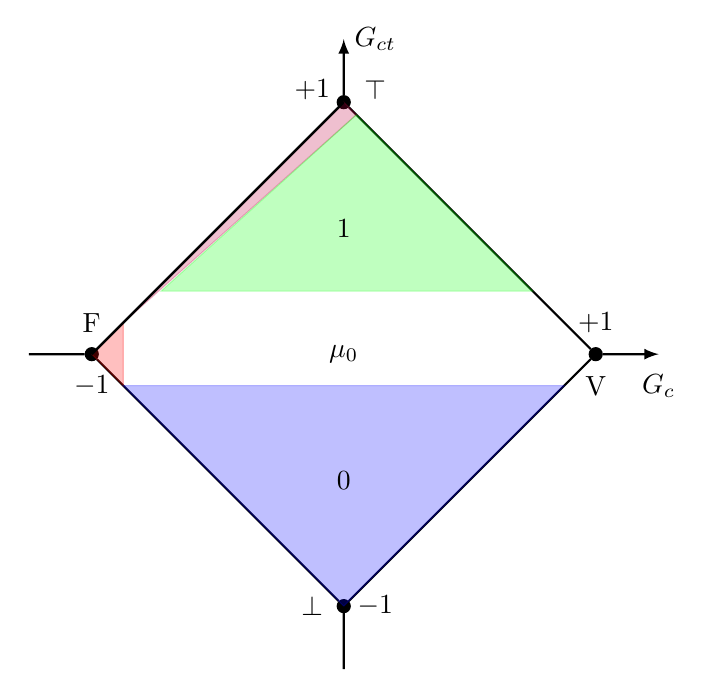
\begin{tikzpicture}[scale=0.80]
\tikzset{ >=latex, inner sep=0pt, outer sep=0pt,  }

%\draw [lightgray, dashed](0,0) grid (10,10);

\node [fill=black, circle] (V) at (9,5) {:};
\node [fill=black, circle] (F) at (1,5) {:};
\node [fill=black, circle] (T) at (5,9) {:};
\node [fill=black, circle] (L) at (5,1) {:};

\draw [->, thick] (V)   -- (10,5);
\draw [    thick] (0,5) -- (F);
\draw [->, thick] (T)   -- (5,10);
\draw [    thick] (5,0) -- (L);

\draw [thick] (V) -- (T);
\draw [thick] (T) -- (F);
\draw [thick] (F) -- (L);
\draw [thick] (L) -- (V);

\node at (10,4.5) {$G_{c}$};
\node at (5.5,10) {$G_{ct}$};

\node at (4.5,9.2) {$+1$};
\node at (9.0,5.5) {$+1$};
\node at (5.5,1.0) {$-1$};
\node at (1.0,4.5) {$-1$};

\node at (9.0,4.5) {V};
\node at (1.0,5.5) {F};
\node at (5.5,9.2) {$\top$};
\node at (4.5,1.0) {$\bot$};

\draw [fill, red,nearly transparent] (1.0,5.0) -- (1.5,5.5) -- (1.5,4.5) -- (1.0,5.0);
\draw [fill, purple, nearly transparent] (1.5,5.5) -- (5.0,9.0) -- (5.2,8.8) -- (1.5,5.5);
\draw [fill, blue, nearly transparent] (5.0,1.0) -- (8.5,4.5) -- (1.5,4.5) -- (5.0,1.0);
\draw [fill, green, nearly transparent] (5.2,8.8) -- (2.1,6.0) -- (8.0,6.0) -- (5.2,8.8);

\draw [thick] (5.0,9.0) -- (1.0,5.0);

\node at (5.0,7.0) {1};
\node at (5.0,5.0) {$\mu_0$};
\node at (5.0,3.0) {0};

\end{tikzpicture}
\label{fig:regiaoAtiva}

{\small Fonte: Próprio autor }
\end{figure}
%%%%%%%%%%%%%%%%%%%%%%%%%%%%%%%%%%%%%%%%%%%%%%%%%%





Os valores de $Gct \ge  0,1$ geram na saída o seu valor máximo,
$1,0$. Desta forma o sistema controlado recebe sinal máximo de
acionamento, gerando a resposta mais rápida possível até que alcance
um grau de contradição menor do que 0,1, correspondente a um erro
menor do que $10\%$.


Na região oposta, para $Gct \le -0,05$ a saída assume
o valor nulo, $0,0$. Assim quando o sistema controlado estiver com
uma velocidade acima do desejado, acima de $5\%$,o desligamento
controlado da saída possibilita a redução mais rápida possível na
velocidade controlada, considerando que não há uma alimentação
reversa para atuar ativamente na redução da velocidade.
 




 
%%% Cap Resultados
%Aplicando um degrau à entrada do sistema, 
%podemos perceber o gráfico da 
%Figura \ref{fig:acaoLPAEtgct100} 
%que o tempo de acomodação é reduzido drasticamente, 
%apesar do sobressinal gerado, 
%este não apresenta problema por estar 
%dentro da tolerância aceitável. 



%%%%%%%%%%%%%%%%%%%%%%%%%%%%%%%%%%%%%%%%%%%%%% Img
%\begin{figure}[!htb]%%%%%%%%%%%%%%%%%%%%%%%%%%%%%%
%\caption{Ação de controle utilizando LPA$E\tau$}
%\vspace{-1cm}\center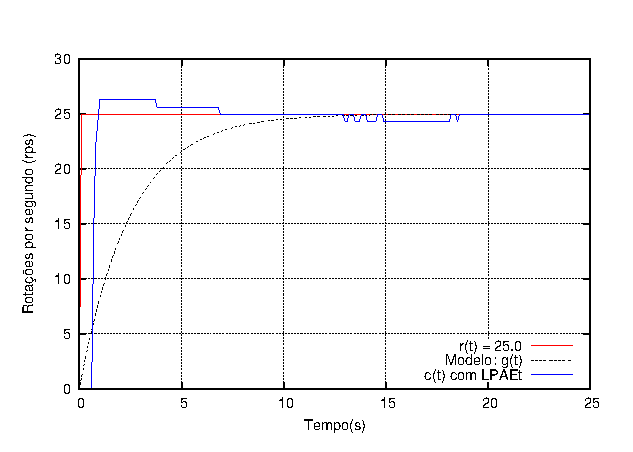
\includegraphics[scale=1.6]{./imagens/LPAEt-gct100.eps}
%\label{fig:acaoLPAEtgct100}

%{\small Fonte: Próprio autor}
%\end{figure}
%%%%%%%%%%%%%%%%%%%%%%%%%%%%%%%%%%%%%%%%%%%%%%%%%%

Considerando a janela entre o $Gct < 0,10$ e $Gct > -0,05$ como a
região em que o controlador irá atuar ativamente, fora do corte e da
saturação, na variável manipilada do sistema controlado.

A variável manipilada assume assim o valor da entrada $\mu_0$,
enviando à saída um valor proporcional ao valor desejado.
Mas como a relação entre o valor de referência e a 
velocidade de rotação do motor não é perfeitamente linear,
para cada região ou patamar da valocidade do motor,
pode haver um erro considerável,
inclusive sendo maior do que o valor permitido pela 
tolerância. 

Assim para reduzir o grau de contradição
em decorrência dessa não linearidade, 
é somado ao $\mu_0$ um valor de correção denominado $\delta$(delta).

Então a representação do reticulado da LPA$E\tau$ 
fica da seguinte forma mostrada na 
Figura \ref{fig:regiaoAtivaMuDelta}. 





%%%%%%%%%%%%%%%%%%%%%%%%%%%%%%%%%%%%%%%%%%%%%% Fig
\begin{figure}[!h]%%%%%%%%%%%%%%%%%%%%%%%%%%%%%%%%
\centering
\caption{Representação da região ativa no reticulado da LPA$E\tau$}
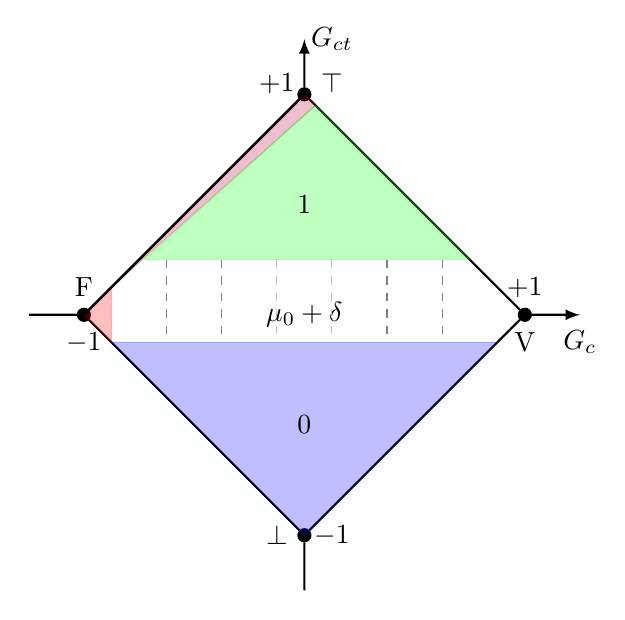
\begin{tikzpicture}[scale=0.70]
\tikzset{ >=latex, inner sep=0pt, outer sep=0pt,  }

%\draw [lightgray, dashed](0,0) grid (10,10);

\node [fill=black, circle] (V) at (9,5) {:};
\node [fill=black, circle] (F) at (1,5) {:};
\node [fill=black, circle] (T) at (5,9) {:};
\node [fill=black, circle] (L) at (5,1) {:};

\draw [->, thick] (V)   -- (10,5);
\draw [    thick] (0,5) -- (F);
\draw [->, thick] (T)   -- (5,10);
\draw [    thick] (5,0) -- (L);

\draw [thick] (V) -- (T);
\draw [thick] (T) -- (F);
\draw [thick] (F) -- (L);
\draw [thick] (L) -- (V);

\node at (10,4.5) {$G_{c}$};
\node at (5.5,10) {$G_{ct}$};

\node at (4.5,9.2) {$+1$};
\node at (9.0,5.5) {$+1$};
\node at (5.5,1.0) {$-1$};
\node at (1.0,4.5) {$-1$};

\node at (9.0,4.5) {V};
\node at (1.0,5.5) {F};
\node at (5.5,9.2) {$\top$};
\node at (4.5,1.0) {$\bot$};

\draw [fill, red,nearly transparent] (1.0,5.0) -- (1.5,5.5) -- (1.5,4.5) -- (1.0,5.0);
\draw [fill, purple, nearly transparent] (1.5,5.5) -- (5.0,9.0) -- (5.2,8.8) -- (1.5,5.5);
\draw [fill, blue, nearly transparent] (5.0,1.0) -- (8.5,4.5) -- (1.5,4.5) -- (5.0,1.0);
\draw [fill, green, nearly transparent] (5.2,8.8) -- (2.1,6.0) -- (8.0,6.0) -- (5.2,8.8);

\draw [thick] (5.0,9.0) -- (1.0,5.0);

\node at (5.0,7.0) {1};
\node at (5.0,5.0) {$\mu_0 + \delta$};
\node at (5.0,3.0) {0};

\draw [dashed, gray] (2.5,6.0) -- (2.5,4.5);
\draw [dashed, gray] (3.5,6.0) -- (3.5,4.5);
\draw [dashed, gray] (6.5,6.0) -- (6.5,4.5);
\draw [dashed, gray] (7.5,6.0) -- (7.5,4.5);
\draw [dashed, lightgray] (4.5,6.0) -- (4.5,4.5);
\draw [dashed, lightgray] (5.5,6.0) -- (5.5,4.5);

\end{tikzpicture}
\label{fig:regiaoAtivaMuDelta}

{\small Fonte: Próprio autor }
\end{figure}
%%%%%%%%%%%%%%%%%%%%%%%%%%%%%%%%%%%%%%%%%%%%%%%%%%





A região ativa então pode ser dividida em 
tantas partes quantas forem necessárias 
para garantir um $\delta$ satisfatório para tal região,
pois esse valor não garante erro nulo para toda extensão
possível.





%######################################
\begin{comment}


\begin{figure}[!h]
\centering
\caption{Representação da região ativa no reticulado da LPA$E\tau$}
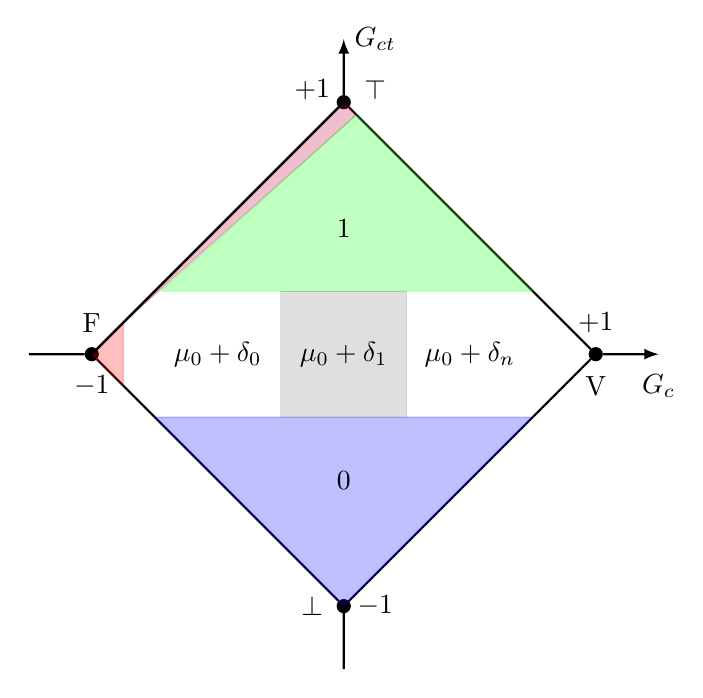
\begin{tikzpicture}[scale=0.80]
\tikzset{ >=latex, inner sep=0pt, outer sep=0pt,  }

%\draw [lightgray, dashed](0,0) grid (10,10);

\node [fill=black, circle] (V) at (9,5) {:};
\node [fill=black, circle] (F) at (1,5) {:};
\node [fill=black, circle] (T) at (5,9) {:};
\node [fill=black, circle] (L) at (5,1) {:};

\draw [->, thick] (V)   -- (10,5);
\draw [    thick] (0,5) -- (F);
\draw [->, thick] (T)   -- (5,10);
\draw [    thick] (5,0) -- (L);

\draw [thick] (V) -- (T);
\draw [thick] (T) -- (F);
\draw [thick] (F) -- (L);
\draw [thick] (L) -- (V);

%\draw[thick] (SW) rectangle (NE);
%\fill[nearly transparent] (SW) rectangle (NE);

\node at (10,4.5) {$G_{c}$};
\node at (5.5,10) {$G_{ct}$};

\node at (4.5,9.2) {$+1$};
\node at (9.0,5.5) {$+1$};
\node at (5.5,1.0) {$-1$};
\node at (1.0,4.5) {$-1$};

\node at (9.0,4.5) {V};
\node at (1.0,5.5) {F};
\node at (5.5,9.2) {$\top$};
\node at (4.5,1.0) {$\bot$};

\draw [fill, red,nearly transparent] (1.0,5.0) -- (1.5,5.5) -- (1.5,4.5) -- (1.0,5.0);
\draw [fill, purple, nearly transparent] (1.5,5.5) -- (5.0,9.0) -- (5.2,8.8) -- (1.5,5.5);
\draw [fill, blue, nearly transparent] (5.0,1.0) -- (8.0,4.0) -- (2.0,4.0) -- (5.0,1.0);
\draw [fill, green, nearly transparent] (5.2,8.8) -- (2.1,6.0) -- (8.0,6.0) -- (5.2,8.8);

\draw [fill, gray, nearly transparent] (4.0,6.0) -- (4.0,4.0)-- (6.0,4.0) -- (6.0,6.0) -- (4.0,6.0);


%\draw [dashed, purple] (5.2,8.8) -- (1.5,5.5);
\draw [thick] (5.0,9.0) -- (1.0,5.0);
%\draw [gray,thick] (V) -- (F);


\node at (5.0,7.0) {1};
\node at (3.0,5.0) {$\mu_0 + \delta_0$};
\node at (5.0,5.0) {$\mu_0 + \delta_1$};
\node at (7.0,5.0) {$\mu_0 + \delta_n$};
\node at (5.0,3.0) {0};

\end{tikzpicture}
\label{fig:regiaoAtivaMuDeltaN}

{\small Fonte: Próprio autor }
\end{figure}


\end{comment}
%######################################



Para gerar um divisão de valores alvo, 
em que o erro seja de no máximo 5\%, 
foi gerada uma tabela que tem como valor inicial
o 10, pois é assumido que para o sistema em estudo,
valores abaixo são considerados zona morta.

A cada incremento de 10\% aproximadamente, 
é gerado o próximo elemento, até o máximo valor menor do que
100, equivalente à 100\% do valor máximo de saída.

Sendo assim segue a 
Tabela \ref{tab:correcaoDelta} 
com os respectivos valores alvo, 
os limites inferiores e superiores, 
que são calculados baseados em decremento de 5\% e
incremento de 5\%, respectivamente, ao valor alvo.

Para todo valor alvo, uma variação positiva ou negativa
de 5\% está enquadrada dentro dos limites motrados na Tabela.

Esses intervalos abrangem todo o intervalo entre 
o valor 10 e o 100, mínimo e máximo, 
de modo a qualquer valor desejado fique 
dentro de algum intervalo, 
e possua um valor alvo bem próximo.


\begin{table}[h]
\centering
\caption{Valores de correção para a condição de contradição}
\label{tab:correcaoDelta}

\begin{tabular}{c|c|c||c}
\hline
%Intervalo de amostras  &  erro médio relativo \\ \hline
Limite Inferior & Alvo & Limite Superior & Valor de Correção\\ \hline
\hline
%0 a 1 $\tau$ & 83,40 \% \\ \hline
 9,5 & 10 & 10,5 & $\delta_0$ \\ \hline
10,5 & 11 & 11,5 & $\delta_1$ \\ \hline
11,5 & 12 & 12,5 & $\delta_2$ \\ \hline
12,5 & 13 & 14,0 & $\delta_3$ \\ \hline
14,0 & 15 & 15,5 & $\delta_4$ \\ \hline
15,5 & 16 & 17,0 & $\delta_5$ \\ \hline
17,0 & 18 & 19,0 & $\delta_6$ \\ \hline
19,0 & 20 & 21,0 & $\delta_7$ \\ \hline
21,0 & 22 & 23,0 & $\delta_8$ \\ \hline
23,4 & 24 & 25,4 & $\delta_9$ \\ \hline
25,4 & 27 & 28,4 & $\delta_{10}$ \\ \hline
28,4 & 30 & 31,4 & $\delta_{11}$ \\ \hline
31,4 & 33 & 34,4 & $\delta_{12}$ \\ \hline
34,4 & 36 & 37,4 & $\delta_{13}$ \\ \hline
37,4 & 39 & 40,9 & $\delta_{14}$ \\ \hline
40,9 & 43 & 44,9 & $\delta_{15}$ \\ \hline
44,9 & 47 & 48,9 & $\delta_{16}$ \\ \hline
48,9 & 51 & 53,4 & $\delta_{17}$ \\ \hline
53,4 & 56 & 58,9 & $\delta_{18}$ \\ \hline
58,9 & 62 & 64,9 & $\delta_{19}$ \\ \hline
64,9 & 68 & 71,3 & $\delta_{20}$ \\ \hline
71,3 & 75 & 78,3 & $\delta_{21}$ \\ \hline
78,3 & 82 & 86,3 & $\delta_{22}$ \\ \hline
86,3 & 91 &100,0 & $\delta_{23}$ \\ \hline

\end{tabular}

{\vspace{0.2cm} \small Fonte: Próprio autor}
\end{table}


Para cada valor alvo, há um valor $\delta$ associado, 
que é um valor de correção.
Tomando como exemplo o valor de referência 25\%, 
no momento inicial há uma grande contradição,
então o reticulado assume na saída o valor 1, 
do estado de valor máximo apresentado na 
Figura \ref{fig:regiaoAtivaMuDelta}.
Ao sistema então é aplicada a potência máxima, 
vencendo a inércia do repouso.
O grau de contradição é reduzido conforme 
o sistema se aproxima do ponto de operação desejado,
e quando o seu valor é menor do que 
o parâmetro de limite, nesse caso estabelecido em 0,10,
a saída assume o valor equivalente ao $\mu_0$, ou seja,
o valor de referência, então: $\mu_0 = 0,25$, porém 
é acrescido o valor do $\delta_9$, 
que refere-se ao intervalo em que se encontra o 25\%.

Assim a saída do controlador LPA$E\tau$ é 
$\mu_0 + \delta_9$
para um valor de referência de 25\% do valor máximo.





%%%%%%%%%%%%%%%%%%%%%%%%%%%%%%%%%%%%%%%%%%%%%%%%%%%%%%%%%%%%
%%%%%%%%%%%%%%%%%%%%%%%%%%%%%%%%%%%%%%%%%%%%%%%%%%%%%%%%%%%%





\section{O fator de correção $\delta$}

O fator de correção $\delta$ tem a finalidade de corrigir a variável
manipilada de modo a zerar a diferença entre a variável controlada e a
variável de referência. A correção aqui empregada é de ajuste fino da
variável manipilada.

A correção se dá por um algorítmo que faz a leitura de forma cíclica
do grau de contradição e atualiza o $\delta$ correspondente ao patamar
em execução.

A dificuldade aqui encontrada é no fato de que a atualização do
$\delta$ somente pode ocorrer após a estabilização do sinal no patamar
após a mudança de velocidade, seja em um primeiro momento de
acionamento com a velocidade saído do zero para um valor desejado de
referência, como entre valores desejados diferentes de zero e
diferentes entre si. 

%Um temporizador é implementado de modo a 
%gerar um primeiro intevalo de 3 segundos para 
%partida e acomodação do sistema, 
%em seguida a cada 1 segundo é feita uma verificação
%do grau de contradição, 
%e como resultado dessa verificação, 
%um incremento do fator de correção $\delta$ 
%que está em operação é realizada. 

Assim, de forma adaptativa, 
os valores de $\delta$ sempre estão sendo atualizados
para variações que possam ocorrer no processo. 

%Caso o tempo de 1 segundo seja muito alto para um 
%determinado processo, 
%para as perturbações envolvidas no processo,
%o tempo pode ser alterado para gerar uma resposta 
%mais rápida ou mais lenta. 




%%%%%%%%%%%%%%%%%%%%%%%%%%%%%%%%%%%%%%%%%%%%%%%%%%%%%%%%%%%%
%%%%%%%%%%%%%%%%%%%%%%%%%%%%%%%%%%%%%%%%%%%%%%%%%%%%%%%%%%%%
